\batchmode
\documentclass[12pt,a4paper]{article}
\RequirePackage{ifthen}


\usepackage{graphicx}
\usepackage{caption}
\usepackage{natbib}
\usepackage{afterpage}

\usepackage{hyperref}
\hypersetup{%
    pdfborder = {0 0 0}
}
\hypersetup{
    colorlinks,
    citecolor=blue,
    filecolor=blue,
    linkcolor=blue,
    urlcolor=blue
}
%
\renewcommand{\familydefault}{\sfdefault}
%
\renewcommand{\captionfont}{\small}


\usepackage{xcolor}

\usepackage[]{inputenc}



\makeatletter
\AtBeginDocument{\makeatletter
\input /home/bp1/sandbox/digital_signal_processing/digital_signal_processing.aux
\makeatother
}

\makeatletter
\count@=\the\catcode`\_ \catcode`\_=8 
\newenvironment{tex2html_wrap}{}{}%
\catcode`\<=12\catcode`\_=\count@
\newcommand{\providedcommand}[1]{\expandafter\providecommand\csname #1\endcsname}%
\newcommand{\renewedcommand}[1]{\expandafter\providecommand\csname #1\endcsname{}%
  \expandafter\renewcommand\csname #1\endcsname}%
\newcommand{\newedenvironment}[1]{\newenvironment{#1}{}{}\renewenvironment{#1}}%
\let\newedcommand\renewedcommand
\let\renewedenvironment\newedenvironment
\makeatother
\let\mathon=$
\let\mathoff=$
\ifx\AtBeginDocument\undefined \newcommand{\AtBeginDocument}[1]{}\fi
\newbox\sizebox
\setlength{\hoffset}{0pt}\setlength{\voffset}{0pt}
\addtolength{\textheight}{\footskip}\setlength{\footskip}{0pt}
\addtolength{\textheight}{\topmargin}\setlength{\topmargin}{0pt}
\addtolength{\textheight}{\headheight}\setlength{\headheight}{0pt}
\addtolength{\textheight}{\headsep}\setlength{\headsep}{0pt}
\setlength{\textwidth}{349pt}
\newwrite\lthtmlwrite
\makeatletter
\let\realnormalsize=\normalsize
\global\topskip=2sp
\def\preveqno{}\let\real@float=\@float \let\realend@float=\end@float
\def\@float{\let\@savefreelist\@freelist\real@float}
\def\liih@math{\ifmmode$\else\bad@math\fi}
\def\end@float{\realend@float\global\let\@freelist\@savefreelist}
\let\real@dbflt=\@dbflt \let\end@dblfloat=\end@float
\let\@largefloatcheck=\relax
\let\if@boxedmulticols=\iftrue
\def\@dbflt{\let\@savefreelist\@freelist\real@dbflt}
\def\adjustnormalsize{\def\normalsize{\mathsurround=0pt \realnormalsize
 \parindent=0pt\abovedisplayskip=0pt\belowdisplayskip=0pt}%
 \def\phantompar{\csname par\endcsname}\normalsize}%
\def\lthtmltypeout#1{{\let\protect\string \immediate\write\lthtmlwrite{#1}}}%
\usepackage[tightpage,active]{preview}
\newbox\lthtmlPageBox
\newdimen\lthtmlCropMarkHeight
\newdimen\lthtmlCropMarkDepth
\long\def\lthtmlTightVBox#1#2{%
    \setbox\lthtmlPageBox\vbox{\hbox{\catcode`\_=8 #2}}%
    \lthtmlCropMarkHeight=\ht\lthtmlPageBox \advance \lthtmlCropMarkHeight 6pt
    \lthtmlCropMarkDepth=\dp\lthtmlPageBox
    \lthtmltypeout{^^J:#1:lthtmlCropMarkHeight:=\the\lthtmlCropMarkHeight}%
    \lthtmltypeout{^^J:#1:lthtmlCropMarkDepth:=\the\lthtmlCropMarkDepth:1ex:=\the \dimexpr 1ex}%
    \begin{preview}\copy\lthtmlPageBox\end{preview}}%
\long\def\lthtmlTightFBox#1#2{%
    \adjustnormalsize\setbox\lthtmlPageBox=\vbox\bgroup %
    \let\ifinner=\iffalse \let\)\liih@math %
    {\catcode`\_=8 #2}%
    \@next\next\@currlist{}{\def\next{\voidb@x}}%
    \expandafter\box\next\egroup %
    \lthtmlCropMarkHeight=\ht\lthtmlPageBox \advance \lthtmlCropMarkHeight 6pt
    \lthtmlCropMarkDepth=\dp\lthtmlPageBox
    \lthtmltypeout{^^J:#1:lthtmlCropMarkHeight:=\the\lthtmlCropMarkHeight}%
    \lthtmltypeout{^^J:#1:lthtmlCropMarkDepth:=\the\lthtmlCropMarkDepth:1ex:=\the \dimexpr 1ex}%
    \begin{preview}\copy\lthtmlPageBox\end{preview}}%
    \long\def\lthtmlinlinemathA#1#2\lthtmlindisplaymathZ{\lthtmlTightVBox{#1}{#2}}
    \def\lthtmlinlineA#1#2\lthtmlinlineZ{\lthtmlTightVBox{#1}{#2}}
    \long\def\lthtmldisplayA#1#2\lthtmldisplayZ{\lthtmlTightVBox{#1}{#2}}
    \long\def\lthtmlinlinemathA#1#2\lthtmlindisplaymathZ{\lthtmlTightVBox{#1}{#2}}
    \def\lthtmlinlineA#1#2\lthtmlinlineZ{\lthtmlTightVBox{#1}{#2}}
    \long\def\lthtmldisplayA#1#2\lthtmldisplayZ{\lthtmlTightVBox{#1}{#2}}
    \long\def\lthtmldisplayB#1#2\lthtmldisplayZ{\\edef\preveqno{(\theequation)}%
        \lthtmlTightVBox{#1}{\let\@eqnnum\relax#2}}
    \long\def\lthtmlfigureA#1#2\lthtmlfigureZ{\let\@savefreelist\@freelist
        \lthtmlTightFBox{#1}{#2}\global\let\@freelist\@savefreelist}
    \long\def\lthtmlpictureA#1#2\lthtmlpictureZ{\let\@savefreelist\@freelist
        \lthtmlTightVBox{#1}{#2}\global\let\@freelist\@savefreelist}
\def\lthtmlcheckvsize{\ifdim\ht\sizebox<\vsize 
  \ifdim\wd\sizebox<\hsize\expandafter\hfill\fi \expandafter\vfill
  \else\expandafter\vss\fi}%
\providecommand{\selectlanguage}[1]{}%
\makeatletter \tracingstats = 1 


\begin{document}
\pagestyle{empty}\thispagestyle{empty}\lthtmltypeout{}%
\lthtmltypeout{latex2htmlLength hsize=\the\hsize}\lthtmltypeout{}%
\lthtmltypeout{latex2htmlLength vsize=\the\vsize}\lthtmltypeout{}%
\lthtmltypeout{latex2htmlLength hoffset=\the\hoffset}\lthtmltypeout{}%
\lthtmltypeout{latex2htmlLength voffset=\the\voffset}\lthtmltypeout{}%
\lthtmltypeout{latex2htmlLength topmargin=\the\topmargin}\lthtmltypeout{}%
\lthtmltypeout{latex2htmlLength topskip=\the\topskip}\lthtmltypeout{}%
\lthtmltypeout{latex2htmlLength headheight=\the\headheight}\lthtmltypeout{}%
\lthtmltypeout{latex2htmlLength headsep=\the\headsep}\lthtmltypeout{}%
\lthtmltypeout{latex2htmlLength parskip=\the\parskip}\lthtmltypeout{}%
\lthtmltypeout{latex2htmlLength oddsidemargin=\the\oddsidemargin}\lthtmltypeout{}%
\makeatletter
\if@twoside\lthtmltypeout{latex2htmlLength evensidemargin=\the\evensidemargin}%
\else\lthtmltypeout{latex2htmlLength evensidemargin=\the\oddsidemargin}\fi%
\lthtmltypeout{}%
\makeatother
\setcounter{page}{1}
\onecolumn

% !!! IMAGES START HERE !!!

{\newpage\clearpage
\lthtmlinlinemathA{tex2html_wrap_inline5707}%
$\Delta $%
\lthtmlindisplaymathZ
\lthtmlcheckvsize\clearpage}

{\newpage\clearpage
\lthtmlinlinemathA{tex2html_wrap_inline5710}%
$t=0$%
\lthtmlindisplaymathZ
\lthtmlcheckvsize\clearpage}

{\newpage\clearpage
\lthtmlinlinemathA{tex2html_wrap_inline5713}%
$F$%
\lthtmlindisplaymathZ
\lthtmlcheckvsize\clearpage}

{\newpage\clearpage
\lthtmlinlinemathA{tex2html_wrap_inline5715}%
$f$%
\lthtmlindisplaymathZ
\lthtmlcheckvsize\clearpage}

{\newpage\clearpage
\lthtmlinlinemathA{tex2html_wrap_inline5717}%
$F_s$%
\lthtmlindisplaymathZ
\lthtmlcheckvsize\clearpage}

{\newpage\clearpage
\lthtmlinlinemathA{tex2html_wrap_inline5722}%
$x(n)$%
\lthtmlindisplaymathZ
\lthtmlcheckvsize\clearpage}

{\newpage\clearpage
\lthtmlinlinemathA{tex2html_wrap_inline5727}%
$X(k)$%
\lthtmlindisplaymathZ
\lthtmlcheckvsize\clearpage}

{\newpage\clearpage
\lthtmlinlinemathA{tex2html_wrap_inline5729}%
$N$%
\lthtmlindisplaymathZ
\lthtmlcheckvsize\clearpage}

{\newpage\clearpage
\lthtmlinlinemathA{tex2html_wrap_inline5731}%
$N/2$%
\lthtmlindisplaymathZ
\lthtmlcheckvsize\clearpage}

{\newpage\clearpage
\lthtmlinlinemathA{tex2html_wrap_inline5733}%
$X(0)$%
\lthtmlindisplaymathZ
\lthtmlcheckvsize\clearpage}

{\newpage\clearpage
\lthtmlinlinemathA{tex2html_wrap_inline5743}%
$t<0$%
\lthtmlindisplaymathZ
\lthtmlcheckvsize\clearpage}

{\newpage\clearpage
\lthtmlinlinemathA{tex2html_wrap_inline5746}%
$t=1$%
\lthtmlindisplaymathZ
\lthtmlcheckvsize\clearpage}

{\newpage\clearpage
\lthtmlinlinemathA{tex2html_wrap_inline5749}%
$w$%
\lthtmlindisplaymathZ
\lthtmlcheckvsize\clearpage}

{\newpage\clearpage
\lthtmlinlinemathA{tex2html_wrap_inline5751}%
$2^w$%
\lthtmlindisplaymathZ
\lthtmlcheckvsize\clearpage}

{\newpage\clearpage
\lthtmlinlinemathA{tex2html_wrap_inline5755}%
$f=0.1$%
\lthtmlindisplaymathZ
\lthtmlcheckvsize\clearpage}

{\newpage\clearpage
\lthtmlinlinemathA{tex2html_wrap_inline5758}%
$\Omega = 2\pi F$%
\lthtmlindisplaymathZ
\lthtmlcheckvsize\clearpage}

{\newpage\clearpage
\lthtmlinlinemathA{tex2html_wrap_inline5764}%
$\omega _0$%
\lthtmlindisplaymathZ
\lthtmlcheckvsize\clearpage}

{\newpage\clearpage
\lthtmlinlinemathA{tex2html_wrap_inline5769}%
$r$%
\lthtmlindisplaymathZ
\lthtmlcheckvsize\clearpage}

{\newpage\clearpage
\lthtmlpictureA{tex2html_wrap5779}%

\includegraphics[width=\textwidth]{SchEng_mono}%
\lthtmlpictureZ
\lthtmlcheckvsize\clearpage}

\stepcounter{section}
\stepcounter{section}
\stepcounter{subsection}
\stepcounter{subsection}
\stepcounter{subsection}
\stepcounter{section}
\stepcounter{subsection}
\stepcounter{paragraph}
\stepcounter{paragraph}
\stepcounter{paragraph}
\stepcounter{subsection}
\stepcounter{subsection}
\stepcounter{paragraph}
{\newpage\clearpage
\lthtmlinlinemathA{tex2html_wrap_inline1767}%
$=6\cdot 10^{23}$%
\lthtmlindisplaymathZ
\lthtmlcheckvsize\clearpage}

\stepcounter{paragraph}
{\newpage\clearpage
\lthtmlinlinemathA{tex2html_wrap_inline1769}%
$1, 2, 3$%
\lthtmlindisplaymathZ
\lthtmlcheckvsize\clearpage}

\stepcounter{paragraph}
\stepcounter{paragraph}
\stepcounter{subsection}
\stepcounter{paragraph}
\stepcounter{paragraph}
\stepcounter{subsection}
\stepcounter{subsection}
\stepcounter{subsection}
\stepcounter{subsection}
\stepcounter{subsection}
\stepcounter{paragraph}
\stepcounter{paragraph}
\stepcounter{section}
{\newpage\clearpage
\lthtmlinlinemathA{tex2html_wrap_indisplay5811}%
$\displaystyle \mbox{Analogue} \rightarrow \mbox{A/D} \rightarrow \mbox{Digital processing}
\rightarrow \mbox{D/A} \rightarrow \mbox{Analogue}
$%
\lthtmlindisplaymathZ
\lthtmlcheckvsize\clearpage}

\stepcounter{subsection}
{\newpage\clearpage
\lthtmlinlinemathA{tex2html_wrap_indisplay5814}%
$\displaystyle \underbrace{X_{a}(nT)}_{\mbox{analogue signal}}~ \equiv \underbrace{x(n)}_{\mbox{discrete data}}
$%
\lthtmlindisplaymathZ
\lthtmlcheckvsize\clearpage}

{\newpage\clearpage
\lthtmlinlinemathA{tex2html_wrap_inline1771}%
$X_a$%
\lthtmlindisplaymathZ
\lthtmlcheckvsize\clearpage}

{\newpage\clearpage
\lthtmlinlinemathA{tex2html_wrap_inline1773}%
$T$%
\lthtmlindisplaymathZ
\lthtmlcheckvsize\clearpage}

{\newpage\clearpage
\lthtmlinlinemathA{tex2html_wrap_inline1775}%
$\frac{1}{T}=F_s$%
\lthtmlindisplaymathZ
\lthtmlcheckvsize\clearpage}

{\newpage\clearpage
\lthtmlinlinemathA{tex2html_wrap_inline1779}%
$X(n) \rightarrow X_{q}(n)$%
\lthtmlindisplaymathZ
\lthtmlcheckvsize\clearpage}

{\newpage\clearpage
\lthtmlinlinemathA{tex2html_wrap_inline1781}%
$X_{q}(n) \rightarrow$%
\lthtmlindisplaymathZ
\lthtmlcheckvsize\clearpage}

\stepcounter{subsection}
\stepcounter{section}
{\newpage\clearpage
\lthtmlinlinemathA{tex2html_wrap_inline1787}%
$X(n)$%
\lthtmlindisplaymathZ
\lthtmlcheckvsize\clearpage}

{\newpage\clearpage
\lthtmlinlinemathA{tex2html_wrap_indisplay5827}%
$\displaystyle X(n) = X_{a}(nT),  \qquad -\infty < n < +\infty
$%
\lthtmlindisplaymathZ
\lthtmlcheckvsize\clearpage}

\stepcounter{subsection}
{\newpage\clearpage
\lthtmlinlinemathA{tex2html_wrap_indisplay5830}%
$\displaystyle F_{s} = \frac{1}{T_s}
$%
\lthtmlindisplaymathZ
\lthtmlcheckvsize\clearpage}

{\newpage\clearpage
\lthtmlinlinemathA{tex2html_wrap_indisplay5832}%
$\displaystyle X_{a}(t) = X_{a}(nT) = X_{a}(\frac{n}{F_{s}})
$%
\lthtmlindisplaymathZ
\lthtmlcheckvsize\clearpage}

{\newpage\clearpage
\lthtmlpictureA{tex2html_wrap5833}%
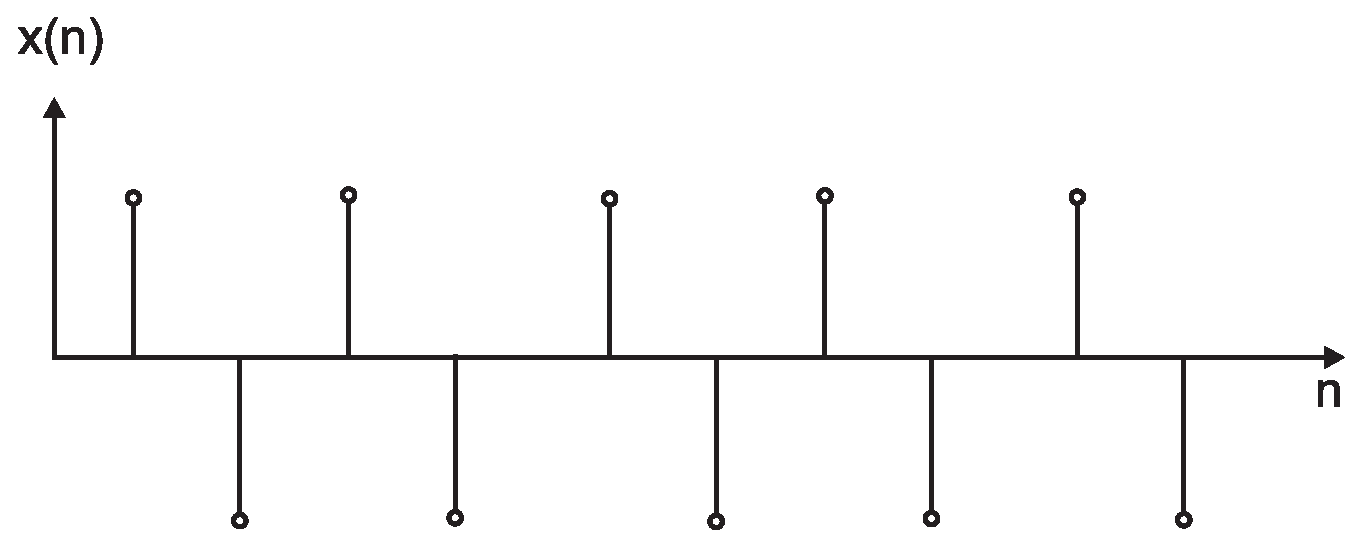
\includegraphics[width=0.75\textwidth]{max_sampl}%
\lthtmlpictureZ
\lthtmlcheckvsize\clearpage}

{\newpage\clearpage
\lthtmlinlinemathA{tex2html_wrap_inline1789}%
$0.5$%
\lthtmlindisplaymathZ
\lthtmlcheckvsize\clearpage}

{\newpage\clearpage
\lthtmlinlinemathA{tex2html_wrap_inline1791}%
$0\ldots 0.5$%
\lthtmlindisplaymathZ
\lthtmlcheckvsize\clearpage}

{\newpage\clearpage
\lthtmlinlinemathA{tex2html_wrap_inline1793}%
$X_{a}(t)$%
\lthtmlindisplaymathZ
\lthtmlcheckvsize\clearpage}

{\newpage\clearpage
\lthtmlinlinemathA{tex2html_wrap_indisplay5842}%
$\displaystyle X_{a}(t) = A\cos (2\pi F t)
$%
\lthtmlindisplaymathZ
\lthtmlcheckvsize\clearpage}

{\newpage\clearpage
\lthtmlinlinemathA{tex2html_wrap_indisplay5844}%
$\displaystyle t = n/F_s
$%
\lthtmlindisplaymathZ
\lthtmlcheckvsize\clearpage}

{\newpage\clearpage
\lthtmlinlinemathA{tex2html_wrap_indisplay5846}%
$\displaystyle X_{a}(n) = A \cos (2 \pi F/F_s n)
$%
\lthtmlindisplaymathZ
\lthtmlcheckvsize\clearpage}

{\newpage\clearpage
\lthtmlinlinemathA{tex2html_wrap_indisplay5848}%
$\displaystyle \mbox{Normalised frequency:} \qquad f =  \frac {F}{F_s}
$%
\lthtmlindisplaymathZ
\lthtmlcheckvsize\clearpage}

{\newpage\clearpage
\lthtmlinlinemathA{tex2html_wrap_inline1799}%
$f_{\mbox{scipy}} =  2 \frac {F}{F_s}$%
\lthtmlindisplaymathZ
\lthtmlcheckvsize\clearpage}

{\newpage\clearpage
\lthtmlinlinemathA{tex2html_wrap_inline1801}%
$f_{\mbox{scipy}}=1$%
\lthtmlindisplaymathZ
\lthtmlcheckvsize\clearpage}

{\newpage\clearpage
\lthtmlinlinemathA{tex2html_wrap_inline1803}%
$f=0.5$%
\lthtmlindisplaymathZ
\lthtmlcheckvsize\clearpage}

\stepcounter{subsection}
{\newpage\clearpage
\lthtmlinlinemathA{tex2html_wrap_indisplay5859}%
$\displaystyle X_{a}(n) = A \cos (2 \pi n f)
$%
\lthtmlindisplaymathZ
\lthtmlcheckvsize\clearpage}

{\newpage\clearpage
\lthtmlinlinemathA{tex2html_wrap_inline1809}%
$n$%
\lthtmlindisplaymathZ
\lthtmlcheckvsize\clearpage}

{\newpage\clearpage
\lthtmlinlinemathA{tex2html_wrap_inline1811}%
$f>0.5$%
\lthtmlindisplaymathZ
\lthtmlcheckvsize\clearpage}

{\newpage\clearpage
\lthtmlinlinemathA{tex2html_wrap_inline1813}%
$f = 1$%
\lthtmlindisplaymathZ
\lthtmlcheckvsize\clearpage}

{\newpage\clearpage
\lthtmlinlinemathA{tex2html_wrap_indisplay5864}%
$\displaystyle X_{a}(n) = \cos (2 \pi n) = 1 \qquad f=1
$%
\lthtmlindisplaymathZ
\lthtmlcheckvsize\clearpage}

{\newpage\clearpage
\lthtmlinlinemathA{tex2html_wrap_inline1815}%
$f = 2, 3, 4, \ldots$%
\lthtmlindisplaymathZ
\lthtmlcheckvsize\clearpage}

{\newpage\clearpage
\lthtmlinlinemathA{tex2html_wrap_inline1821}%
$F/F_s$%
\lthtmlindisplaymathZ
\lthtmlcheckvsize\clearpage}

{\newpage\clearpage
\lthtmlinlinemathA{tex2html_wrap_inline1825}%
$\frac{1}{2} F_s$%
\lthtmlindisplaymathZ
\lthtmlcheckvsize\clearpage}

{\newpage\clearpage
\lthtmlinlinemathA{tex2html_wrap_inline1827}%
$0\ldots \frac{1}{2} F_s$%
\lthtmlindisplaymathZ
\lthtmlcheckvsize\clearpage}

{\newpage\clearpage
\lthtmlinlinemathA{tex2html_wrap_inline1829}%
$f=0\ldots 0.5$%
\lthtmlindisplaymathZ
\lthtmlcheckvsize\clearpage}

{\newpage\clearpage
\lthtmlinlinemathA{tex2html_wrap_inline1831}%
$B$%
\lthtmlindisplaymathZ
\lthtmlcheckvsize\clearpage}

{\newpage\clearpage
\lthtmlinlinemathA{tex2html_wrap_indisplay5876}%
$\displaystyle B < \frac{1}{2}F_s
$%
\lthtmlindisplaymathZ
\lthtmlcheckvsize\clearpage}

{\newpage\clearpage
\lthtmlpictureA{tex2html_wrap5878}%
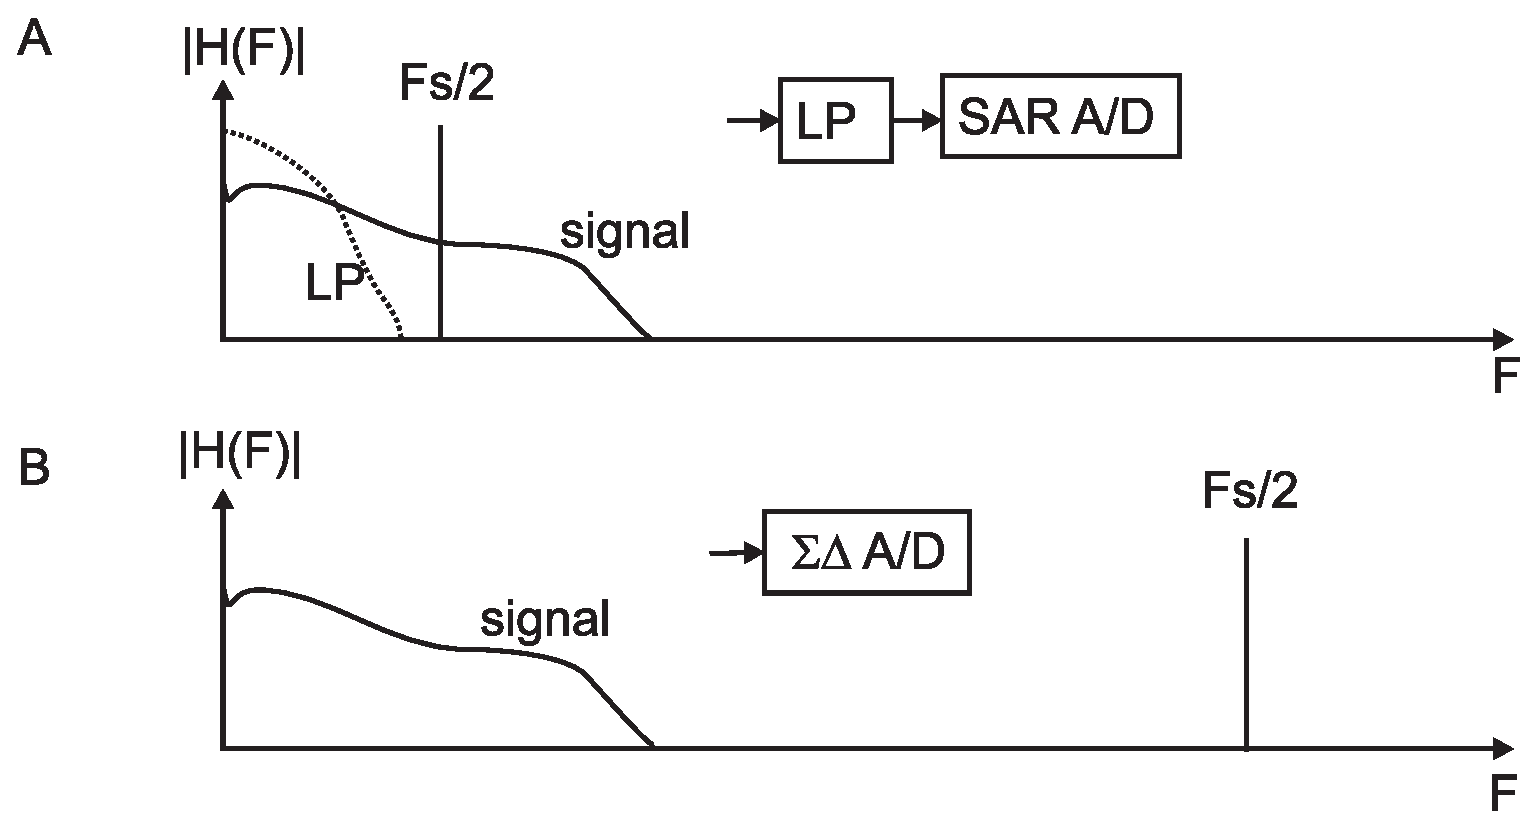
\includegraphics[width=0.75\textwidth]{anti_alias}%
\lthtmlpictureZ
\lthtmlcheckvsize\clearpage}

\stepcounter{subsection}
{\newpage\clearpage
\lthtmlinlinemathA{tex2html_wrap_indisplay5885}%
$\displaystyle F_s > 2 F_{\mbox{max}}
$%
\lthtmlindisplaymathZ
\lthtmlcheckvsize\clearpage}

{\newpage\clearpage
\lthtmlinlinemathA{tex2html_wrap_inline1839}%
$F_{\mbox{max}}$%
\lthtmlindisplaymathZ
\lthtmlcheckvsize\clearpage}

{\newpage\clearpage
\lthtmlinlinemathA{tex2html_wrap_indisplay5888}%
$\displaystyle x_{a}(t) = \sum_{i=1}^{n} A_i \cos (2 \pi F_{i}t  + \Theta_{i})
$%
\lthtmlindisplaymathZ
\lthtmlcheckvsize\clearpage}

{\newpage\clearpage
\lthtmlinlinemathA{tex2html_wrap_inline1841}%
$x_{a}(t)$%
\lthtmlindisplaymathZ
\lthtmlcheckvsize\clearpage}

{\newpage\clearpage
\lthtmlinlinemathA{tex2html_wrap_indisplay5891}%
$\displaystyle g(t) = \frac{\sin 2\pi Bt}{2 \pi Bt}
$%
\lthtmlindisplaymathZ
\lthtmlcheckvsize\clearpage}

{\newpage\clearpage
\lthtmlinlinemathA{tex2html_wrap_indisplay5893}%
$\displaystyle B = F_{\mbox{max}}
$%
\lthtmlindisplaymathZ
\lthtmlcheckvsize\clearpage}

{\newpage\clearpage
\lthtmlinlinemathA{tex2html_wrap_indisplay5895}%
$\displaystyle x_{a}(t) = \sum_{h= -a}^{a}x_{a}(\frac{n}{F_s})g(t - \frac{h}{F_s})
$%
\lthtmlindisplaymathZ
\lthtmlcheckvsize\clearpage}

{\newpage\clearpage
\lthtmlpictureA{tex2html_wrap5896}%
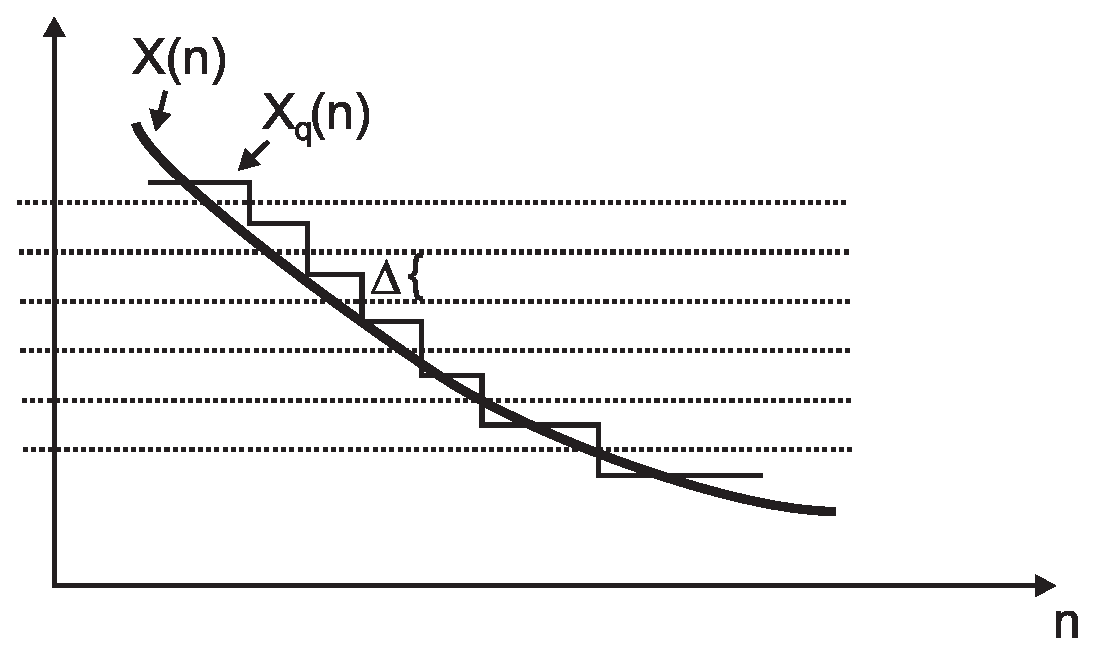
\includegraphics[width=0.75\textwidth]{quant_overv}%
\lthtmlpictureZ
\lthtmlcheckvsize\clearpage}

\stepcounter{section}
{\newpage\clearpage
\lthtmlinlinemathA{tex2html_wrap_indisplay5904}%
$\displaystyle \Delta = \mbox{quantisation step} = 
\frac{x_{\mbox{max}} - x_{\mbox{min}}}{L - 1}
$%
\lthtmlindisplaymathZ
\lthtmlcheckvsize\clearpage}

{\newpage\clearpage
\lthtmlinlinemathA{tex2html_wrap_inline1845}%
$x_{\mbox{max}} - x_{\mbox{min}}$%
\lthtmlindisplaymathZ
\lthtmlcheckvsize\clearpage}

{\newpage\clearpage
\lthtmlinlinemathA{tex2html_wrap_inline1847}%
$4.096V$%
\lthtmlindisplaymathZ
\lthtmlcheckvsize\clearpage}

{\newpage\clearpage
\lthtmlinlinemathA{tex2html_wrap_inline1849}%
$L$%
\lthtmlindisplaymathZ
\lthtmlcheckvsize\clearpage}

{\newpage\clearpage
\lthtmlinlinemathA{tex2html_wrap_indisplay5910}%
$\displaystyle x_{q}(n) = Q[x(n)]
$%
\lthtmlindisplaymathZ
\lthtmlcheckvsize\clearpage}

\stepcounter{subsection}
{\newpage\clearpage
\lthtmlpictureA{tex2html_wrap5912}%
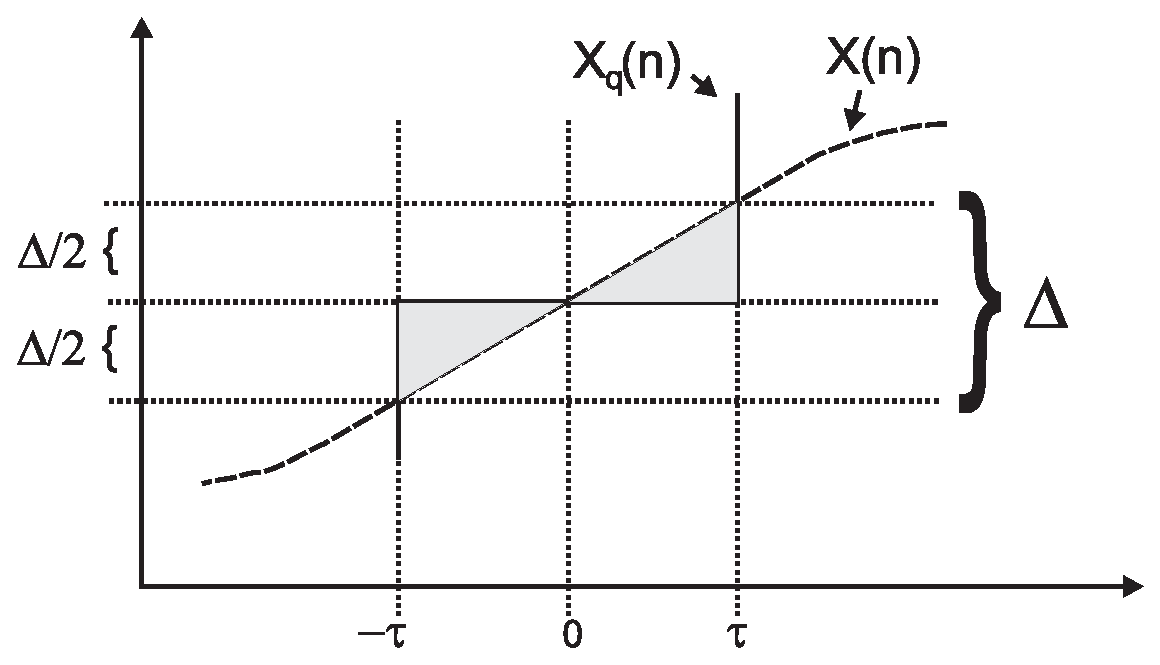
\includegraphics[width=0.75\textwidth]{quant_err}%
\lthtmlpictureZ
\lthtmlcheckvsize\clearpage}

{\newpage\clearpage
\lthtmlinlinemathA{tex2html_wrap_indisplay5919}%
$\displaystyle - \frac{\Delta}{2} \le e(n) \le \frac{\Delta}{2}
$%
\lthtmlindisplaymathZ
\lthtmlcheckvsize\clearpage}

{\newpage\clearpage
\lthtmlinlinemathA{tex2html_wrap_inline1857}%
$P_{q}$%
\lthtmlindisplaymathZ
\lthtmlcheckvsize\clearpage}

{\newpage\clearpage
\lthtmlinlinemathA{tex2html_wrap_indisplay5923}%
$\displaystyle P_{q} = \frac {1}{\tau} \int_{0}^{\tau} e_{q}^{2}(t)  dt
$%
\lthtmlindisplaymathZ
\lthtmlcheckvsize\clearpage}

{\newpage\clearpage
\lthtmlinlinemathA{tex2html_wrap_indisplay5925}%
$\displaystyle P_{q}$%
\lthtmlindisplaymathZ
\lthtmlcheckvsize\clearpage}

{\newpage\clearpage
\lthtmlinlinemathA{tex2html_wrap_indisplay5926}%
$\textstyle =$%
\lthtmlindisplaymathZ
\lthtmlcheckvsize\clearpage}

{\newpage\clearpage
\lthtmlinlinemathA{tex2html_wrap_indisplay5927}%
$\displaystyle \frac{1}{\tau} \int_0^\tau \left(\frac{\Delta}{2\tau}\right)^2 t^2 dt$%
\lthtmlindisplaymathZ
\lthtmlcheckvsize\clearpage}

{\newpage\clearpage
\lthtmlinlinemathA{tex2html_wrap_indisplay5929}%
$\displaystyle \frac{\Delta^2}{4 \tau^3} \int_0^\tau t^2 dt$%
\lthtmlindisplaymathZ
\lthtmlcheckvsize\clearpage}

{\newpage\clearpage
\lthtmlinlinemathA{tex2html_wrap_indisplay5931}%
$\displaystyle P_{q} = \frac{\Delta^2}{12\tau^3} \tau^3 =\frac{\Delta^2}{12}$%
\lthtmlindisplaymathZ
\lthtmlcheckvsize\clearpage}

{\newpage\clearpage
\lthtmlinlinemathA{tex2html_wrap_indisplay5933}%
$\displaystyle P_x = \frac{1}{T_p} \int_{0}^{T_p}(A \cos \Omega t)^2 dt = \frac{A^2}{2}
$%
\lthtmlindisplaymathZ
\lthtmlcheckvsize\clearpage}

{\newpage\clearpage
\lthtmlinlinemathA{tex2html_wrap_indisplay5935}%
$\displaystyle \mbox {SQNR}$%
\lthtmlindisplaymathZ
\lthtmlcheckvsize\clearpage}

{\newpage\clearpage
\lthtmlinlinemathA{tex2html_wrap_indisplay5937}%
$\displaystyle \frac {P_x}{P_q} = \frac{A^2}{2} . \frac{12}{\Delta^2}$%
\lthtmlindisplaymathZ
\lthtmlcheckvsize\clearpage}

{\newpage\clearpage
\lthtmlinlinemathA{tex2html_wrap_indisplay5939}%
$\displaystyle \frac{6A^2}{\Delta^2}$%
\lthtmlindisplaymathZ
\lthtmlcheckvsize\clearpage}

\stepcounter{section}
{\newpage\clearpage
\lthtmlinlinemathA{tex2html_wrap_inline1859}%
$X(F)$%
\lthtmlindisplaymathZ
\lthtmlcheckvsize\clearpage}

{\newpage\clearpage
\lthtmlinlinemathA{tex2html_wrap_inline1861}%
$x(t)$%
\lthtmlindisplaymathZ
\lthtmlcheckvsize\clearpage}

\stepcounter{subsection}
\stepcounter{subsubsection}
{\newpage\clearpage
\lthtmlinlinemathA{tex2html_wrap_indisplay5946}%
$\displaystyle x(t) = \sum_{k = -\infty}^{\infty} c_{k} e^{j2\pi k F_1 t}
$%
\lthtmlindisplaymathZ
\lthtmlcheckvsize\clearpage}

{\newpage\clearpage
\lthtmlinlinemathA{tex2html_wrap_inline1863}%
$F_1$%
\lthtmlindisplaymathZ
\lthtmlcheckvsize\clearpage}

{\newpage\clearpage
\lthtmlinlinemathA{tex2html_wrap_inline1865}%
$k \neq 1$%
\lthtmlindisplaymathZ
\lthtmlcheckvsize\clearpage}

{\newpage\clearpage
\lthtmlinlinemathA{tex2html_wrap_inline1867}%
$c_k$%
\lthtmlindisplaymathZ
\lthtmlcheckvsize\clearpage}

{\newpage\clearpage
\lthtmlinlinemathA{tex2html_wrap_inline1869}%
$c_1$%
\lthtmlindisplaymathZ
\lthtmlcheckvsize\clearpage}

{\newpage\clearpage
\lthtmlinlinemathA{tex2html_wrap_inline1871}%
$1$%
\lthtmlindisplaymathZ
\lthtmlcheckvsize\clearpage}

{\newpage\clearpage
\lthtmlinlinemathA{tex2html_wrap_inline1873}%
$c_{k}$%
\lthtmlindisplaymathZ
\lthtmlcheckvsize\clearpage}

{\newpage\clearpage
\lthtmlinlinemathA{tex2html_wrap_indisplay5955}%
$\displaystyle c_{k} = \frac{1}{T_p} \int_{T_p} x(t) e^{-j2 \pi k F_1 t} dt
$%
\lthtmlindisplaymathZ
\lthtmlcheckvsize\clearpage}

{\newpage\clearpage
\lthtmlinlinemathA{tex2html_wrap_indisplay5959}%
$\displaystyle c_{k} = c_{- k}^{*} \qquad \Leftrightarrow \qquad x(t)\mbox{ is real}
$%
\lthtmlindisplaymathZ
\lthtmlcheckvsize\clearpage}

{\newpage\clearpage
\lthtmlinlinemathA{tex2html_wrap_indisplay5961}%
$\displaystyle c_{k}$%
\lthtmlindisplaymathZ
\lthtmlcheckvsize\clearpage}

{\newpage\clearpage
\lthtmlinlinemathA{tex2html_wrap_indisplay5963}%
$\displaystyle \mid c_k \mid e^{j \theta_k}$%
\lthtmlindisplaymathZ
\lthtmlcheckvsize\clearpage}

{\newpage\clearpage
\lthtmlinlinemathA{tex2html_wrap_indisplay5964}%
$\displaystyle c_{-k}$%
\lthtmlindisplaymathZ
\lthtmlcheckvsize\clearpage}

{\newpage\clearpage
\lthtmlinlinemathA{tex2html_wrap_indisplay5966}%
$\displaystyle \mid c_k \mid e^{-j \theta_k}$%
\lthtmlindisplaymathZ
\lthtmlcheckvsize\clearpage}

{\newpage\clearpage
\lthtmlinlinemathA{tex2html_wrap_indisplay5968}%
$\displaystyle \cos z = \frac{1}{2} \left(e^{zi} + e^{-zi}\right)
$%
\lthtmlindisplaymathZ
\lthtmlcheckvsize\clearpage}

{\newpage\clearpage
\lthtmlinlinemathA{tex2html_wrap_indisplay5970}%
$\displaystyle x(t)$%
\lthtmlindisplaymathZ
\lthtmlcheckvsize\clearpage}

{\newpage\clearpage
\lthtmlinlinemathA{tex2html_wrap_indisplay5972}%
$\displaystyle c_0 + \sum_{k = 1}^{\infty} \mid c_k \mid e^{j \theta_k} e^{j 2\pi k F_1 t}
+ \sum_{k = 1}^{\infty} \mid c_{k}\mid e^{-j \theta_k} e^{-j 2\pi k F_1 t}$%
\lthtmlindisplaymathZ
\lthtmlcheckvsize\clearpage}

{\newpage\clearpage
\lthtmlinlinemathA{tex2html_wrap_indisplay5974}%
$\displaystyle c_0 + 2 \sum_{k = 1}^{\infty} \mid c_k \mid \cos(2 \pi k F_1 t + \theta_{k})$%
\lthtmlindisplaymathZ
\lthtmlcheckvsize\clearpage}

{\newpage\clearpage
\lthtmlinlinemathA{tex2html_wrap_inline1881}%
$P_{k} = \mid c_{k} \mid^{2}$%
\lthtmlindisplaymathZ
\lthtmlcheckvsize\clearpage}

{\newpage\clearpage
\lthtmlinlinemathA{tex2html_wrap_inline1883}%
$\frac{1}{T_1} = F_1$%
\lthtmlindisplaymathZ
\lthtmlcheckvsize\clearpage}

{\newpage\clearpage
\lthtmlinlinemathA{tex2html_wrap_inline1885}%
$c_{-k} = c_{k}^{*}$%
\lthtmlindisplaymathZ
\lthtmlcheckvsize\clearpage}

\stepcounter{subsubsection}
{\newpage\clearpage
\lthtmlinlinemathA{tex2html_wrap_inline1887}%
$X(t)$%
\lthtmlindisplaymathZ
\lthtmlcheckvsize\clearpage}

{\newpage\clearpage
\lthtmlinlinemathA{tex2html_wrap_indisplay5981}%
$\displaystyle X(F) = \int_{-\infty}^{\infty} x(t) e^{-j 2 \pi F t} dt
$%
\lthtmlindisplaymathZ
\lthtmlcheckvsize\clearpage}

{\newpage\clearpage
\lthtmlinlinemathA{tex2html_wrap_indisplay5984}%
$\displaystyle x(t) = \frac{1}{2\pi} \int_{-\infty}^{\infty} X(F) e^{j 2 \pi F t} dF
$%
\lthtmlindisplaymathZ
\lthtmlcheckvsize\clearpage}

\stepcounter{subsection}
\stepcounter{subsubsection}
{\newpage\clearpage
\lthtmlinlinemathA{tex2html_wrap_indisplay5989}%
$\displaystyle X(\omega)=\sum_{n=-\infty}^{\infty} x(n) e^{-j\omega n}
$%
\lthtmlindisplaymathZ
\lthtmlcheckvsize\clearpage}

{\newpage\clearpage
\lthtmlinlinemathA{tex2html_wrap_indisplay5991}%
$\displaystyle x(n)$%
\lthtmlindisplaymathZ
\lthtmlcheckvsize\clearpage}

{\newpage\clearpage
\lthtmlinlinemathA{tex2html_wrap_indisplay5993}%
$\displaystyle \frac{1}{2\pi} \int_{-\pi}^{\pi} X(\omega) e^{j\omega n} d\omega$%
\lthtmlindisplaymathZ
\lthtmlcheckvsize\clearpage}

{\newpage\clearpage
\lthtmlinlinemathA{tex2html_wrap_indisplay5995}%
$\displaystyle \frac{1}{2\pi} \int_{-0.5}^{0.5} X(f) e^{j 2\pi f n} dt$%
\lthtmlindisplaymathZ
\lthtmlcheckvsize\clearpage}

{\newpage\clearpage
\lthtmlpictureA{tex2html_wrap5997}%
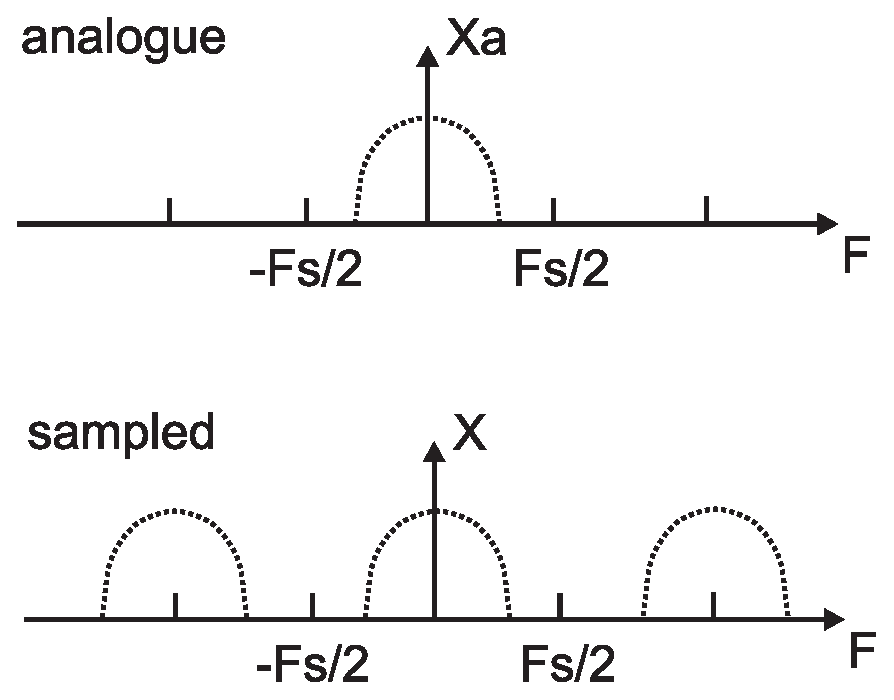
\includegraphics[width=0.75\textwidth]{periodic_ny}%
\lthtmlpictureZ
\lthtmlcheckvsize\clearpage}

\stepcounter{subsubsection}
{\newpage\clearpage
\lthtmlinlinemathA{tex2html_wrap_inline1895}%
$X_a(F)$%
\lthtmlindisplaymathZ
\lthtmlcheckvsize\clearpage}

{\newpage\clearpage
\lthtmlinlinemathA{tex2html_wrap_indisplay6009}%
$\displaystyle X(F) \Leftrightarrow X_a(F)
$%
\lthtmlindisplaymathZ
\lthtmlcheckvsize\clearpage}

{\newpage\clearpage
\lthtmlinlinemathA{tex2html_wrap_indisplay6014}%
$\displaystyle \int_{-0.5}^{0.5} \underbrace{X(f)}_{\mbox{sampled}} e^{j 2 \pi f n} df = 
\int_{-\infty}^{+\infty} \underbrace{X_a(F)}_{\mbox{cont}} e^{j 2\pi n F/F_s} dF
$%
\lthtmlindisplaymathZ
\lthtmlcheckvsize\clearpage}

{\newpage\clearpage
\lthtmlinlinemathA{tex2html_wrap_inline1909}%
$X(f)$%
\lthtmlindisplaymathZ
\lthtmlcheckvsize\clearpage}

{\newpage\clearpage
\lthtmlinlinemathA{tex2html_wrap_inline1911}%
$f=F/F_s$%
\lthtmlindisplaymathZ
\lthtmlcheckvsize\clearpage}

{\newpage\clearpage
\lthtmlinlinemathA{tex2html_wrap_indisplay6018}%
$\displaystyle \frac{1}{F_s} \int_{-F_s/2}^{F_s/2} X(\frac{F}{F_s}) e^{j 2 \pi n F/F_s} dF
=
\int_{-\infty}^{+\infty} X_a(F) e^{j 2\pi n F/F_s} dF
$%
\lthtmlindisplaymathZ
\lthtmlcheckvsize\clearpage}

{\newpage\clearpage
\lthtmlinlinemathA{tex2html_wrap_indisplay6021}%
$\displaystyle \int_{-\infty}^{+\infty} X_a(F) e^{j 2\pi n \frac{F}{F_s}} dF$%
\lthtmlindisplaymathZ
\lthtmlcheckvsize\clearpage}

{\newpage\clearpage
\lthtmlinlinemathA{tex2html_wrap_indisplay6023}%
$\displaystyle \sum_{k=-\infty}^{\infty} \int_{-\frac{1}{2} F_s + k F_s}^{+\frac{1}{2} F_s + k F_s} X_a(F) e^{j2\pi n \frac{F}{F_s}} dF$%
\lthtmlindisplaymathZ
\lthtmlcheckvsize\clearpage}

{\newpage\clearpage
\lthtmlinlinemathA{tex2html_wrap_indisplay6025}%
$\displaystyle \sum_{k=-\infty}^{\infty} \int_{-\frac{1}{2} F_s}^{+\frac{1}{2} F_s} X_a(F-k F_s) \underbrace{e^{j2\pi n\frac{F}{F_s}}}_{k F_s \mbox{ omit.}} dF$%
\lthtmlindisplaymathZ
\lthtmlcheckvsize\clearpage}

{\newpage\clearpage
\lthtmlinlinemathA{tex2html_wrap_indisplay6027}%

% latex2html id marker 6027
$\displaystyle \int_{-\frac{1}{2} F_s}^{+\frac{1}{2} F_s} \underbrace{\sum_{k=-\infty}^{\infty} X_a(F-k F_s)}_{=X(F) \mbox{ of Eq.~\ref{sampl_ana_dig}}} e^{j2\pi n\frac{F}{F_s}} dF$%
\lthtmlindisplaymathZ
\lthtmlcheckvsize\clearpage}

{\newpage\clearpage
\lthtmlinlinemathA{tex2html_wrap_indisplay6029}%
$\displaystyle X(F/F_s)$%
\lthtmlindisplaymathZ
\lthtmlcheckvsize\clearpage}

{\newpage\clearpage
\lthtmlinlinemathA{tex2html_wrap_indisplay6031}%
$\displaystyle F_s \sum_{k=-\infty}^{\infty} X_a(F-kF_s)$%
\lthtmlindisplaymathZ
\lthtmlcheckvsize\clearpage}

{\newpage\clearpage
\lthtmlinlinemathA{tex2html_wrap_indisplay6032}%
$\displaystyle X(f)$%
\lthtmlindisplaymathZ
\lthtmlcheckvsize\clearpage}

{\newpage\clearpage
\lthtmlinlinemathA{tex2html_wrap_indisplay6034}%
$\displaystyle F_s \sum_{k=-\infty}^{\infty} X_a[(f-k)F_s]$%
\lthtmlindisplaymathZ
\lthtmlcheckvsize\clearpage}

{\newpage\clearpage
\lthtmlinlinemathA{tex2html_wrap_inline1921}%
$F_s/2$%
\lthtmlindisplaymathZ
\lthtmlcheckvsize\clearpage}

{\newpage\clearpage
\lthtmlinlinemathA{tex2html_wrap_inline1923}%
$-F/2 \ldots F/2$%
\lthtmlindisplaymathZ
\lthtmlcheckvsize\clearpage}

{\newpage\clearpage
\lthtmlinlinemathA{tex2html_wrap_inline1925}%
$-F/2
+ 34 \ldots F/2 +34$%
\lthtmlindisplaymathZ
\lthtmlcheckvsize\clearpage}

{\newpage\clearpage
\lthtmlpictureA{tex2html_wrap6043}%
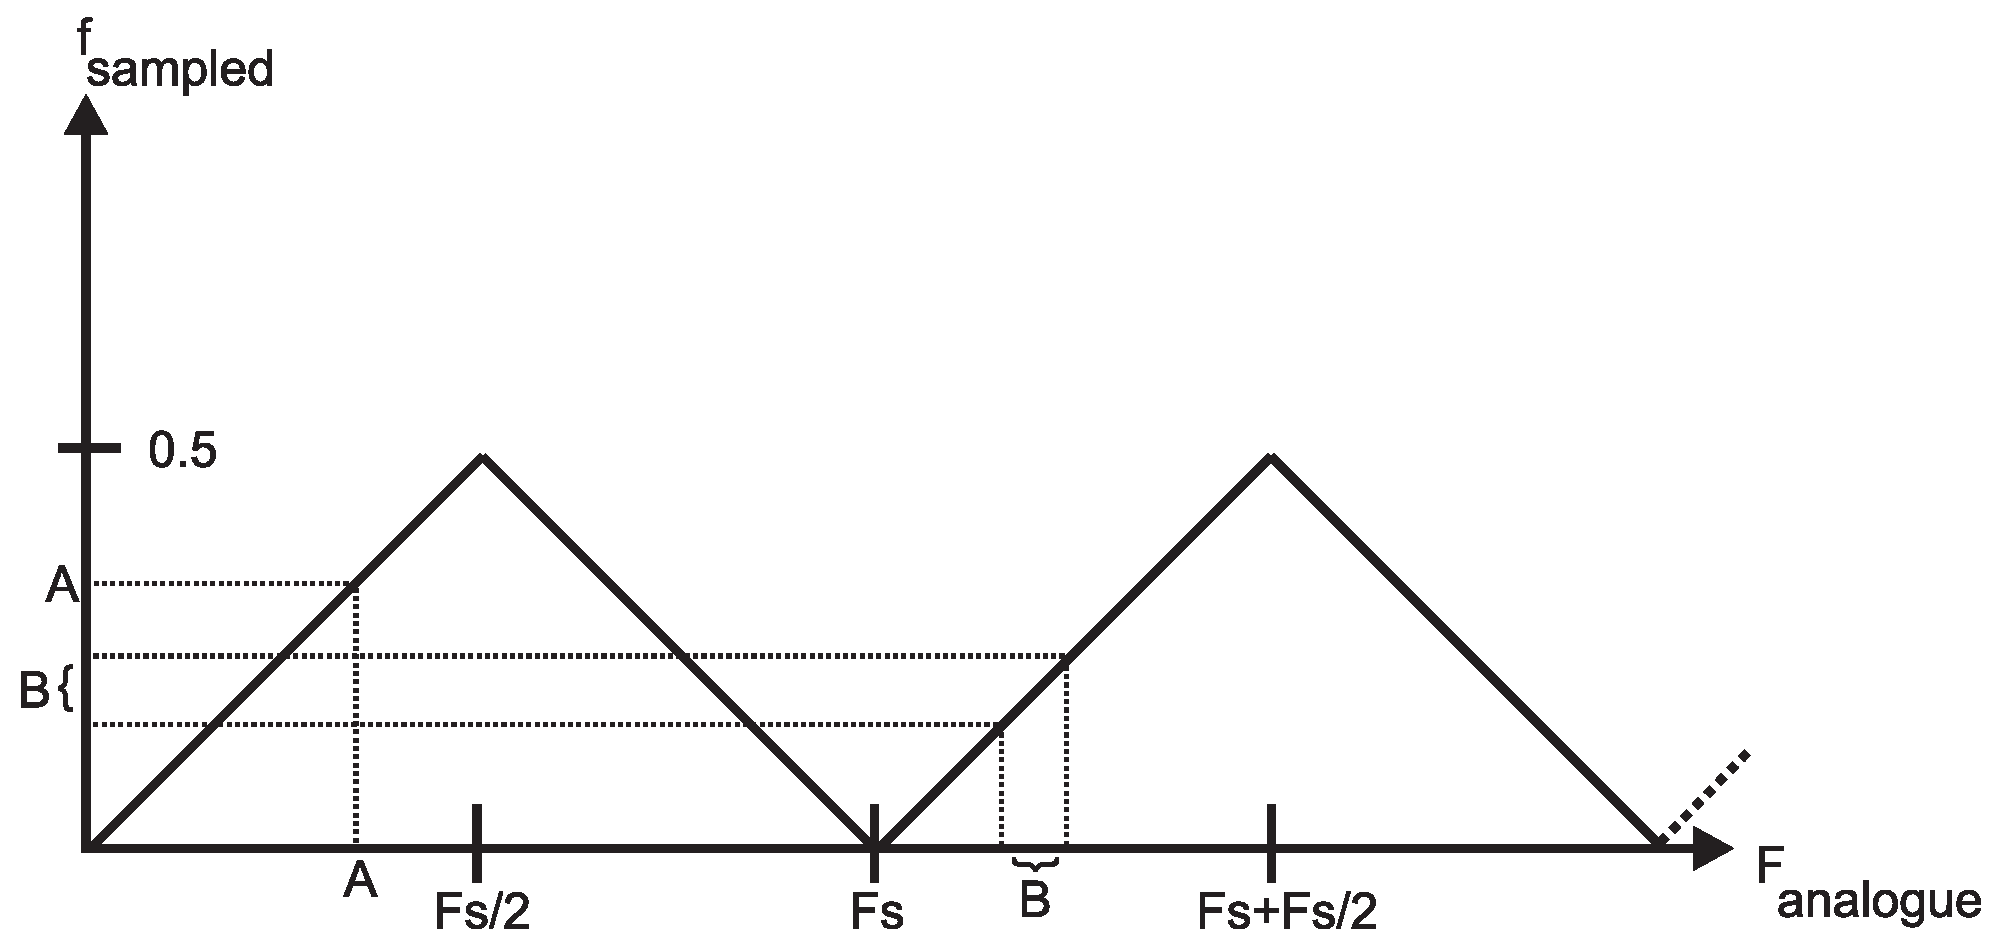
\includegraphics[width=\textwidth]{fold_down}%
\lthtmlpictureZ
\lthtmlcheckvsize\clearpage}

{\newpage\clearpage
\lthtmlinlinemathA{tex2html_wrap_inline1937}%
$F_\textrm{analogue}$%
\lthtmlindisplaymathZ
\lthtmlcheckvsize\clearpage}

{\newpage\clearpage
\lthtmlinlinemathA{tex2html_wrap_inline1939}%
$f_\textrm{sampled}$%
\lthtmlindisplaymathZ
\lthtmlcheckvsize\clearpage}

{\newpage\clearpage
\lthtmlinlinemathA{tex2html_wrap_inline1949}%
$F_s \ldots F_s + 1/2 F_s$%
\lthtmlindisplaymathZ
\lthtmlcheckvsize\clearpage}

{\newpage\clearpage
\lthtmlinlinemathA{tex2html_wrap_inline1953}%
$F_s = 2B$%
\lthtmlindisplaymathZ
\lthtmlcheckvsize\clearpage}

\stepcounter{subsubsection}
{\newpage\clearpage
\lthtmlinlinemathA{tex2html_wrap_indisplay6064}%
$\displaystyle X(k) = \sum_{n=0}^{N-1} x(n) e^{-j2\pi kn / N} \qquad k=0,1,2, \ldots, N-1
$%
\lthtmlindisplaymathZ
\lthtmlcheckvsize\clearpage}

{\newpage\clearpage
\lthtmlinlinemathA{tex2html_wrap_indisplay6067}%
$\displaystyle x(n) = \frac{1}{N} \sum_{k=0}^{N-1} X(k) e^{j 2\pi kn/N} \qquad n=0,1,2,\ldots, N-1
$%
\lthtmlindisplaymathZ
\lthtmlcheckvsize\clearpage}

{\newpage\clearpage
\lthtmlpictureA{tex2html_wrap6068}%
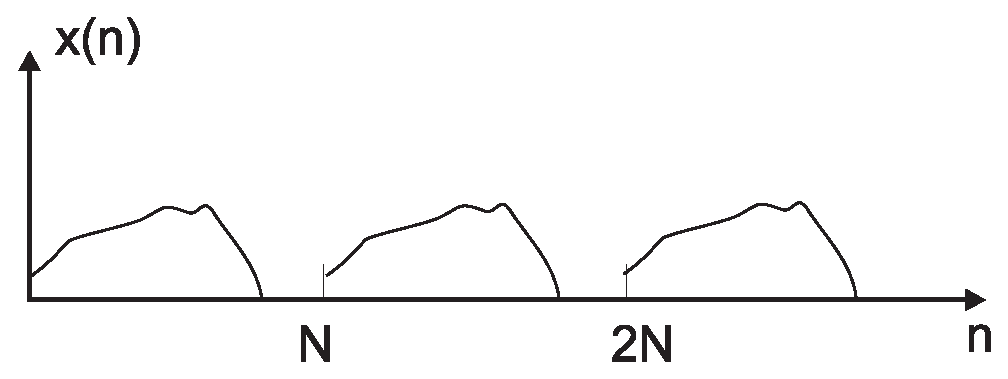
\includegraphics[width=0.75\textwidth]{time_alias}%
\lthtmlpictureZ
\lthtmlcheckvsize\clearpage}

{\newpage\clearpage
\lthtmlinlinemathA{tex2html_wrap_indisplay6077}%
$\displaystyle X\left(\frac{2\pi}{N}k\right) = \sum_{n = -\infty}^{\infty} x(n) e^{-j\frac{2\pi}{N}kn} \qquad k = 0, \ldots, N-1
$%
\lthtmlindisplaymathZ
\lthtmlcheckvsize\clearpage}

{\newpage\clearpage
\lthtmlinlinemathA{tex2html_wrap_indisplay6080}%
$\displaystyle X\left(\frac{2\pi}{N}k\right)$%
\lthtmlindisplaymathZ
\lthtmlcheckvsize\clearpage}

{\newpage\clearpage
\lthtmlinlinemathA{tex2html_wrap_indisplay6082}%
$\displaystyle \sum_{l = -\infty}^{\infty} \sum_{n=lN}^{lN+N-1} x(n)e^{-j \frac{2\pi}{N}kn}$%
\lthtmlindisplaymathZ
\lthtmlcheckvsize\clearpage}

{\newpage\clearpage
\lthtmlinlinemathA{tex2html_wrap_indisplay6084}%
$\displaystyle \sum_{l=-\infty}^{\infty} \sum_{n=0}^{N-1} x(n-lN) e^{-j \frac{2\pi}{N} kn}$%
\lthtmlindisplaymathZ
\lthtmlcheckvsize\clearpage}

{\newpage\clearpage
\lthtmlinlinemathA{tex2html_wrap_indisplay6086}%
$\displaystyle \sum_{n=0}^{N-1} \underbrace{\sum_{l=-\infty}^{\infty} x(n - lN)}_{\mbox{Periodic repetition!}} e^{-j \frac{2\pi}{N}kn}$%
\lthtmlindisplaymathZ
\lthtmlcheckvsize\clearpage}

{\newpage\clearpage
\lthtmlpictureA{tex2html_wrap6088}%
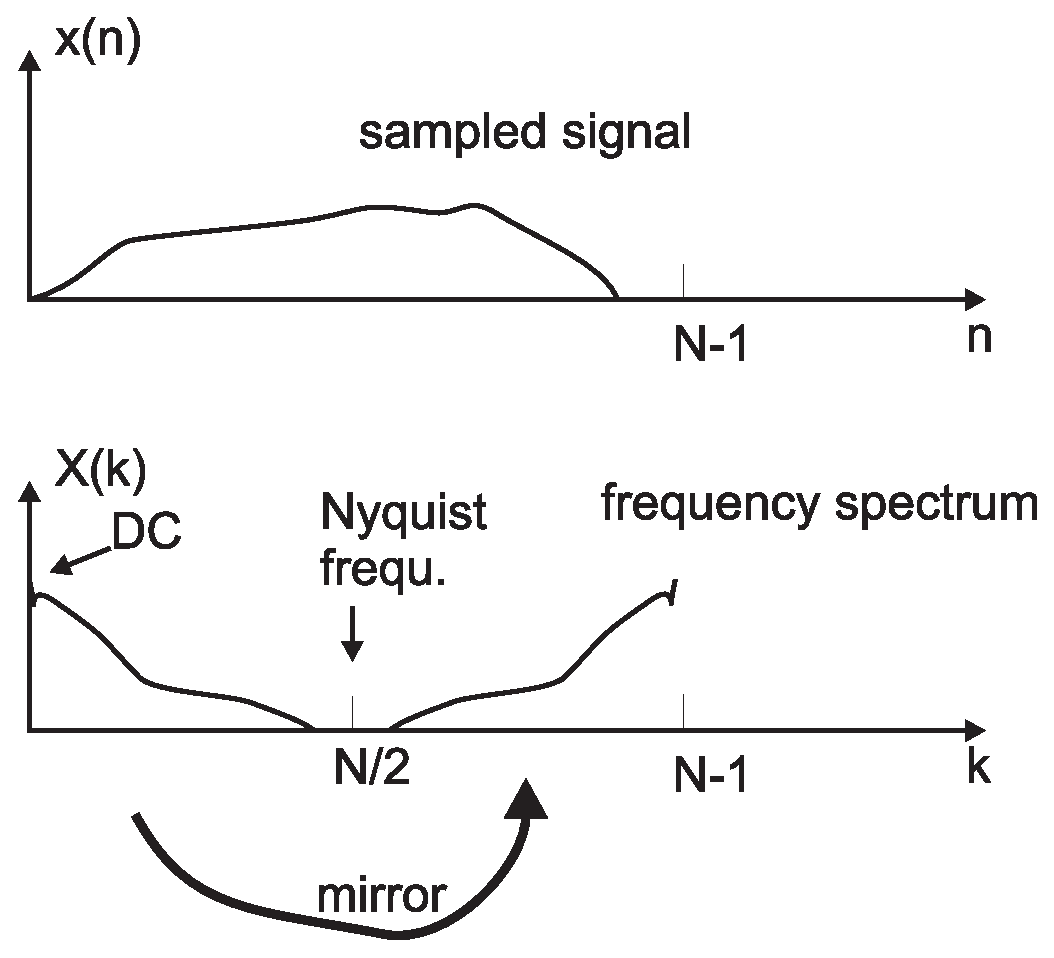
\includegraphics[width=0.75\textwidth]{dft_example}%
\lthtmlpictureZ
\lthtmlcheckvsize\clearpage}

{\newpage\clearpage
\lthtmlinlinemathA{tex2html_wrap_inline1979}%
$X(N/2)$%
\lthtmlindisplaymathZ
\lthtmlcheckvsize\clearpage}

{\newpage\clearpage
\lthtmlinlinemathA{tex2html_wrap_inline1987}%
$y$%
\lthtmlindisplaymathZ
\lthtmlcheckvsize\clearpage}

\stepcounter{subsubsection}
{\newpage\clearpage
\lthtmlinlinemathA{tex2html_wrap_indisplay6112}%
$\displaystyle x(n + N)$%
\lthtmlindisplaymathZ
\lthtmlcheckvsize\clearpage}

{\newpage\clearpage
\lthtmlinlinemathA{tex2html_wrap_indisplay6115}%
$\displaystyle X(k + N)$%
\lthtmlindisplaymathZ
\lthtmlcheckvsize\clearpage}

{\newpage\clearpage
\lthtmlinlinemathA{tex2html_wrap_indisplay6117}%
$\displaystyle X(k)$%
\lthtmlindisplaymathZ
\lthtmlcheckvsize\clearpage}

{\newpage\clearpage
\lthtmlinlinemathA{tex2html_wrap_indisplay6120}%
$\displaystyle x(n)\mbox{ is real} \Leftrightarrow X^*(k) = X(-k) = X(N-k)
$%
\lthtmlindisplaymathZ
\lthtmlcheckvsize\clearpage}

{\newpage\clearpage
\lthtmlinlinemathA{tex2html_wrap_indisplay6124}%
$\textstyle \leftrightarrow$%
\lthtmlindisplaymathZ
\lthtmlcheckvsize\clearpage}

{\newpage\clearpage
\lthtmlinlinemathA{tex2html_wrap_indisplay6126}%
$\displaystyle x(-n)$%
\lthtmlindisplaymathZ
\lthtmlcheckvsize\clearpage}

{\newpage\clearpage
\lthtmlinlinemathA{tex2html_wrap_indisplay6128}%
$\displaystyle X(N - k)$%
\lthtmlindisplaymathZ
\lthtmlcheckvsize\clearpage}

{\newpage\clearpage
\lthtmlinlinemathA{tex2html_wrap_indisplay6130}%
$\displaystyle X_{1}(k) X_{2}(k) \leftrightarrow x_1(n) * x_2(n)
$%
\lthtmlindisplaymathZ
\lthtmlcheckvsize\clearpage}

{\newpage\clearpage
\lthtmlinlinemathA{tex2html_wrap_indisplay6132}%
$\displaystyle x_{3}(m) = \sum_{n = 0}^{N - 1} x_{1}(n) x_{2}(m - n)
$%
\lthtmlindisplaymathZ
\lthtmlcheckvsize\clearpage}

{\newpage\clearpage
\lthtmlpictureA{tex2html_wrap6133}%
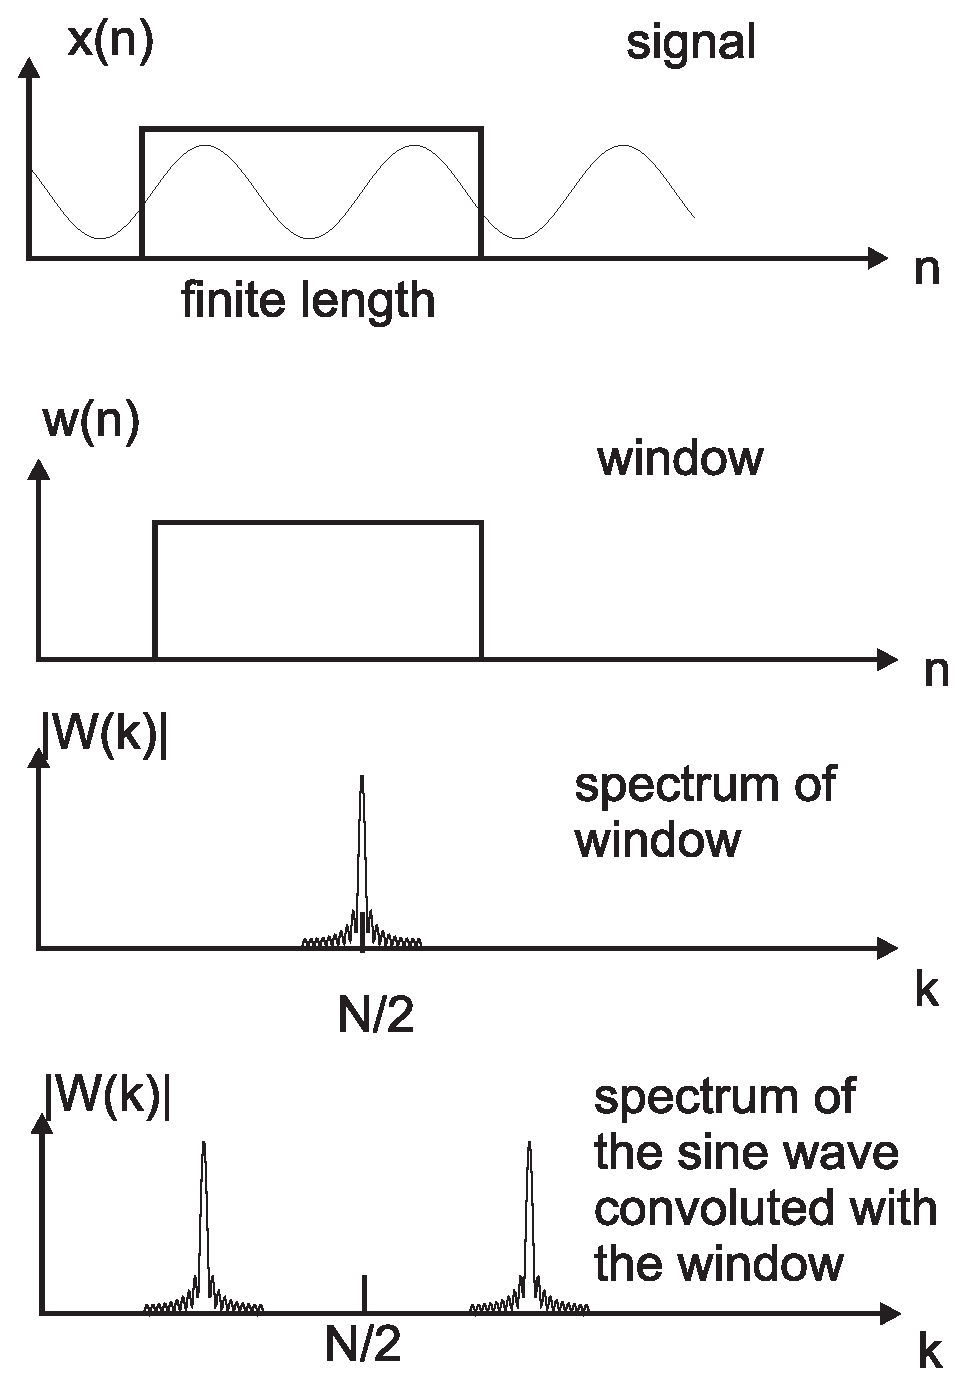
\includegraphics[width=0.75\textwidth]{windowing_dft}%
\lthtmlpictureZ
\lthtmlcheckvsize\clearpage}

\stepcounter{subsubsection}
{\newpage\clearpage
\lthtmlinlinemathA{tex2html_wrap_indisplay6139}%
$\displaystyle x_w(n) = x(n) \cdot w(n)
$%
\lthtmlindisplaymathZ
\lthtmlcheckvsize\clearpage}

{\newpage\clearpage
\lthtmlinlinemathA{tex2html_wrap_inline1993}%
$x$%
\lthtmlindisplaymathZ
\lthtmlcheckvsize\clearpage}

{\newpage\clearpage
\lthtmlinlinemathA{tex2html_wrap_inline1995}%
$w(n)$%
\lthtmlindisplaymathZ
\lthtmlcheckvsize\clearpage}

{\newpage\clearpage
\lthtmlinlinemathA{tex2html_wrap_inline1999}%
$n=0$%
\lthtmlindisplaymathZ
\lthtmlcheckvsize\clearpage}

{\newpage\clearpage
\lthtmlinlinemathA{tex2html_wrap_inline2001}%
$n=L-1$%
\lthtmlindisplaymathZ
\lthtmlcheckvsize\clearpage}

{\newpage\clearpage
\lthtmlinlinemathA{tex2html_wrap_inline2007}%
$x(n) = \cos \omega_0 n$%
\lthtmlindisplaymathZ
\lthtmlcheckvsize\clearpage}

{\newpage\clearpage
\lthtmlinlinemathA{tex2html_wrap_inline2009}%
$-\omega$%
\lthtmlindisplaymathZ
\lthtmlcheckvsize\clearpage}

{\newpage\clearpage
\lthtmlinlinemathA{tex2html_wrap_inline2011}%
$+\omega$%
\lthtmlindisplaymathZ
\lthtmlcheckvsize\clearpage}

{\newpage\clearpage
\lthtmlinlinemathA{tex2html_wrap_indisplay6152}%
$\displaystyle W(\omega) = \frac{sin(\omega L /2)}{sin (\omega / 2)} e^{-j\omega (L -1)/2}
$%
\lthtmlindisplaymathZ
\lthtmlcheckvsize\clearpage}

{\newpage\clearpage
\lthtmlinlinemathA{tex2html_wrap_indisplay6154}%
$\displaystyle X_{3}(\omega) = X(\omega) * W(\omega)
$%
\lthtmlindisplaymathZ
\lthtmlcheckvsize\clearpage}

{\newpage\clearpage
\lthtmlinlinemathA{tex2html_wrap_inline2015}%
$X(\omega)$%
\lthtmlindisplaymathZ
\lthtmlcheckvsize\clearpage}

{\newpage\clearpage
\lthtmlinlinemathA{tex2html_wrap_inline2017}%
$X_{3}(\omega)$%
\lthtmlindisplaymathZ
\lthtmlcheckvsize\clearpage}

{\newpage\clearpage
\lthtmlinlinemathA{tex2html_wrap_inline2019}%
$W(\omega)$%
\lthtmlindisplaymathZ
\lthtmlcheckvsize\clearpage}

\stepcounter{subsubsection}
{\newpage\clearpage
\lthtmlinlinemathA{tex2html_wrap_indisplay6162}%
$\displaystyle X(k) = \sum_{n = 0}^{N-1}  x(n) W_{N}^{kn}
$%
\lthtmlindisplaymathZ
\lthtmlcheckvsize\clearpage}

{\newpage\clearpage
\lthtmlinlinemathA{tex2html_wrap_indisplay6164}%
$\displaystyle W_{N} = e^{-j 2\pi/N}
$%
\lthtmlindisplaymathZ
\lthtmlcheckvsize\clearpage}

{\newpage\clearpage
\lthtmlinlinemathA{tex2html_wrap_inline2025}%
$N^2$%
\lthtmlindisplaymathZ
\lthtmlcheckvsize\clearpage}

{\newpage\clearpage
\lthtmlinlinemathA{tex2html_wrap_indisplay6167}%
$\textstyle x(2m)$%
\lthtmlindisplaymathZ
\lthtmlcheckvsize\clearpage}

{\newpage\clearpage
\lthtmlinlinemathA{tex2html_wrap_indisplay6168}%
$\textstyle x(2m + 1),$%
\lthtmlindisplaymathZ
\lthtmlcheckvsize\clearpage}

{\newpage\clearpage
\lthtmlinlinemathA{tex2html_wrap_indisplay6169}%
$\displaystyle \qquad m = 0, ..... , \frac{N}{2} - 1$%
\lthtmlindisplaymathZ
\lthtmlcheckvsize\clearpage}

{\newpage\clearpage
\lthtmlinlinemathA{tex2html_wrap_inline2027}%
$W_N^{2mk} = W_{N/2}^{mk}$%
\lthtmlindisplaymathZ
\lthtmlcheckvsize\clearpage}

{\newpage\clearpage
\lthtmlinlinemathA{tex2html_wrap_indisplay6174}%
$\displaystyle \sum_{m=0}^{N/2-1} x(2m) W_{N}^{2mk} + \sum_{m=0}^{N/2 - 1}  x(2m + 1) W_{N}^{k (2m + 1)}$%
\lthtmlindisplaymathZ
\lthtmlcheckvsize\clearpage}

{\newpage\clearpage
\lthtmlinlinemathA{tex2html_wrap_indisplay6176}%
$\displaystyle \sum_{m=0}^{N/2-1} x(2m) W_{N/2}^{mk} + W_{N}^{k} \sum_{m = 0}^{N/2 - 1} x(2m + 1) W_{N/2}^{mk}$%
\lthtmlindisplaymathZ
\lthtmlcheckvsize\clearpage}

{\newpage\clearpage
\lthtmlinlinemathA{tex2html_wrap_indisplay6178}%
$\displaystyle F_{e}(k) + W_{N}^{k} F_{o}(k)$%
\lthtmlindisplaymathZ
\lthtmlcheckvsize\clearpage}

{\newpage\clearpage
\lthtmlinlinemathA{tex2html_wrap_inline2029}%
$F_e$%
\lthtmlindisplaymathZ
\lthtmlcheckvsize\clearpage}

{\newpage\clearpage
\lthtmlinlinemathA{tex2html_wrap_inline2031}%
$F_o$%
\lthtmlindisplaymathZ
\lthtmlcheckvsize\clearpage}

{\newpage\clearpage
\lthtmlinlinemathA{tex2html_wrap_inline2033}%
$(N/2)^2$%
\lthtmlindisplaymathZ
\lthtmlcheckvsize\clearpage}

{\newpage\clearpage
\lthtmlinlinemathA{tex2html_wrap_inline2035}%
$2 \cdot (N/2)^2 = \frac{N^2}{2}$%
\lthtmlindisplaymathZ
\lthtmlcheckvsize\clearpage}

{\newpage\clearpage
\lthtmlinlinemathA{tex2html_wrap_inline2037}%
$F_{e}(k)$%
\lthtmlindisplaymathZ
\lthtmlcheckvsize\clearpage}

{\newpage\clearpage
\lthtmlinlinemathA{tex2html_wrap_inline2039}%
$F_{o}(k)$%
\lthtmlindisplaymathZ
\lthtmlcheckvsize\clearpage}

{\newpage\clearpage
\lthtmlinlinemathA{tex2html_wrap_inline2041}%
$F_{ee}(k), F_{eo}(k), F_{oe}(k)$%
\lthtmlindisplaymathZ
\lthtmlcheckvsize\clearpage}

{\newpage\clearpage
\lthtmlinlinemathA{tex2html_wrap_inline2043}%
$F_{oo}(k)$%
\lthtmlindisplaymathZ
\lthtmlcheckvsize\clearpage}

{\newpage\clearpage
\lthtmlpictureA{tex2html_wrap6187}%
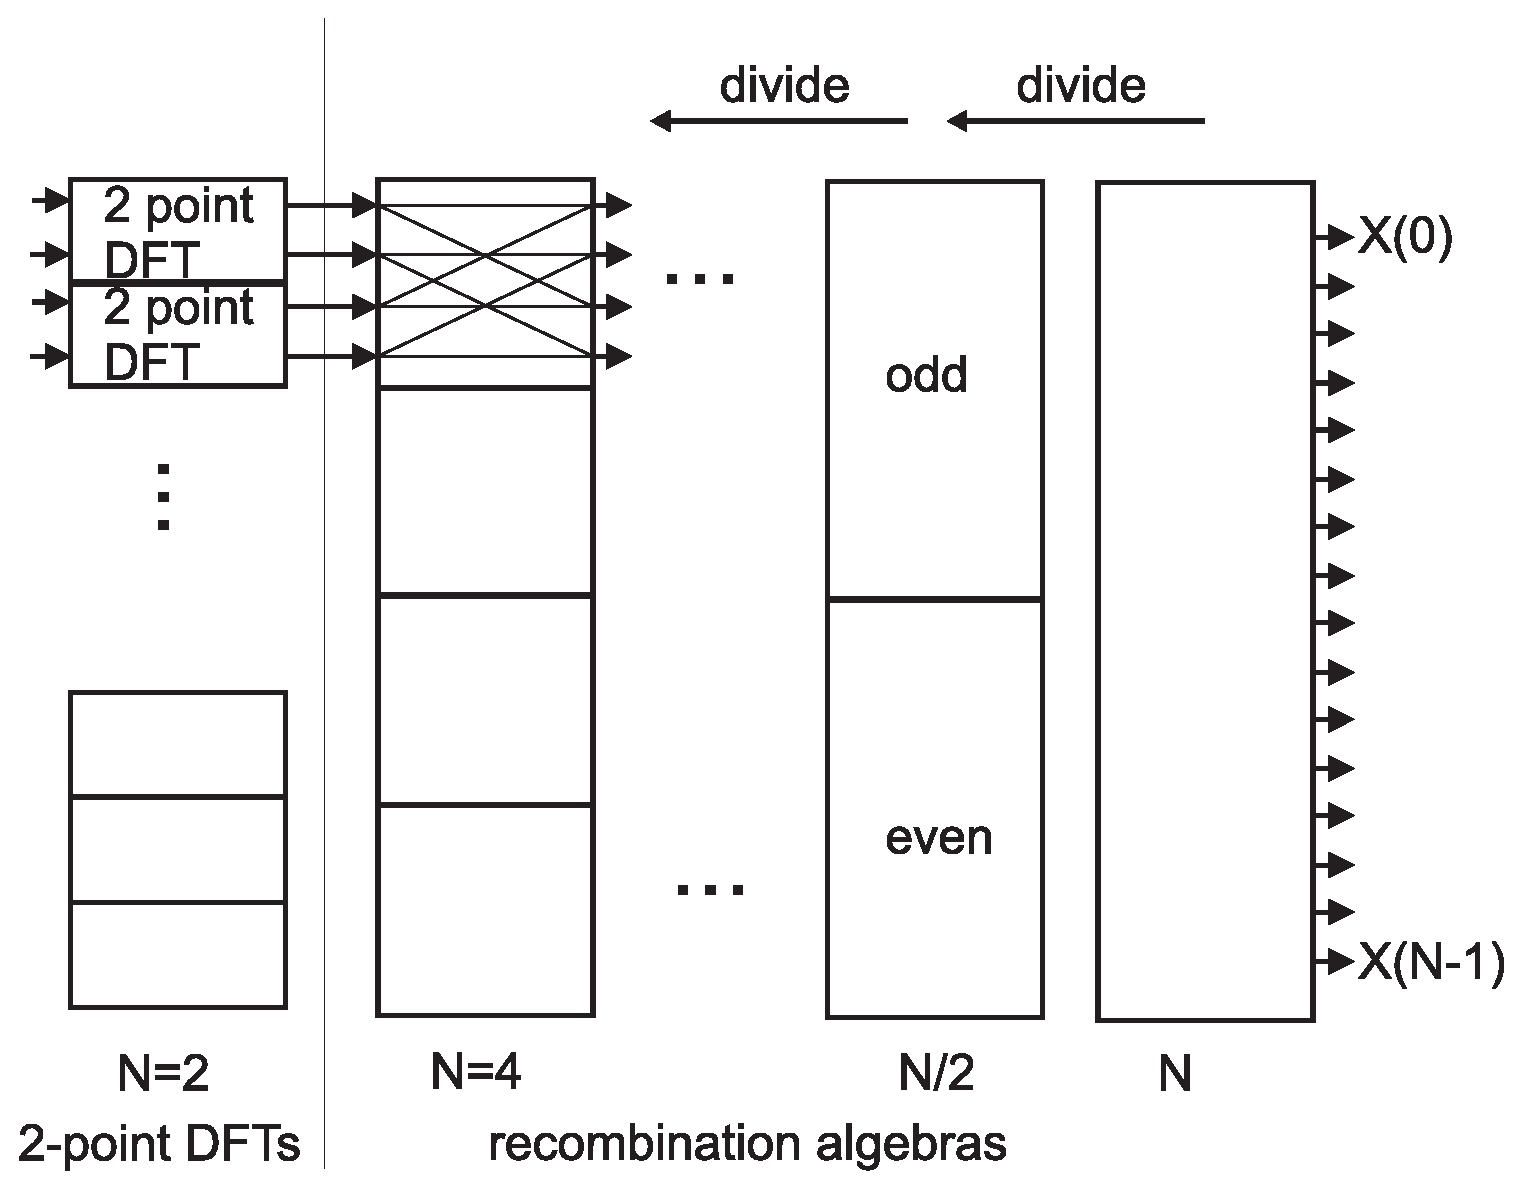
\includegraphics[width=0.75\textwidth]{fft_div}%
\lthtmlpictureZ
\lthtmlcheckvsize\clearpage}

{\newpage\clearpage
\lthtmlinlinemathA{tex2html_wrap_indisplay6194}%
$\displaystyle X_{i}(k) = X_{ie}(k) + W_{L}^{k} X_{io}(k)
$%
\lthtmlindisplaymathZ
\lthtmlcheckvsize\clearpage}

{\newpage\clearpage
\lthtmlinlinemathA{tex2html_wrap_inline2047}%
$W_{L}^{k}$%
\lthtmlindisplaymathZ
\lthtmlcheckvsize\clearpage}

{\newpage\clearpage
\lthtmlinlinemathA{tex2html_wrap_inline2049}%
$N=2$%
\lthtmlindisplaymathZ
\lthtmlcheckvsize\clearpage}

{\newpage\clearpage
\lthtmlinlinemathA{tex2html_wrap_indisplay6198}%
$\displaystyle \mbox{DC:} \qquad X(0)$%
\lthtmlindisplaymathZ
\lthtmlcheckvsize\clearpage}

{\newpage\clearpage
\lthtmlinlinemathA{tex2html_wrap_indisplay6200}%
$\displaystyle x(0) + \underbrace{W_2^0}_{1} x(1) = x(0) + x(1)$%
\lthtmlindisplaymathZ
\lthtmlcheckvsize\clearpage}

{\newpage\clearpage
\lthtmlinlinemathA{tex2html_wrap_indisplay6201}%
$\displaystyle \mbox{Nyquist frequ.:} \qquad X(1)$%
\lthtmlindisplaymathZ
\lthtmlcheckvsize\clearpage}

{\newpage\clearpage
\lthtmlinlinemathA{tex2html_wrap_indisplay6203}%
$\displaystyle x(0) + \underbrace{W_2^1}_{-1} x(1) = x(0) - x(1)$%
\lthtmlindisplaymathZ
\lthtmlcheckvsize\clearpage}

{\newpage\clearpage
\lthtmlinlinemathA{tex2html_wrap_inline2051}%
$1,-1,1,-1,\ldots$%
\lthtmlindisplaymathZ
\lthtmlcheckvsize\clearpage}

{\newpage\clearpage
\lthtmlinlinemathA{tex2html_wrap_inline2055}%
$N
\log_2 N$%
\lthtmlindisplaymathZ
\lthtmlcheckvsize\clearpage}

{\newpage\clearpage
\lthtmlinlinemathA{tex2html_wrap_inline2059}%
$1,-1,j,-j$%
\lthtmlindisplaymathZ
\lthtmlcheckvsize\clearpage}

\stepcounter{subsection}
{\newpage\clearpage
\lthtmlpictureA{tex2html_wrap6210}%
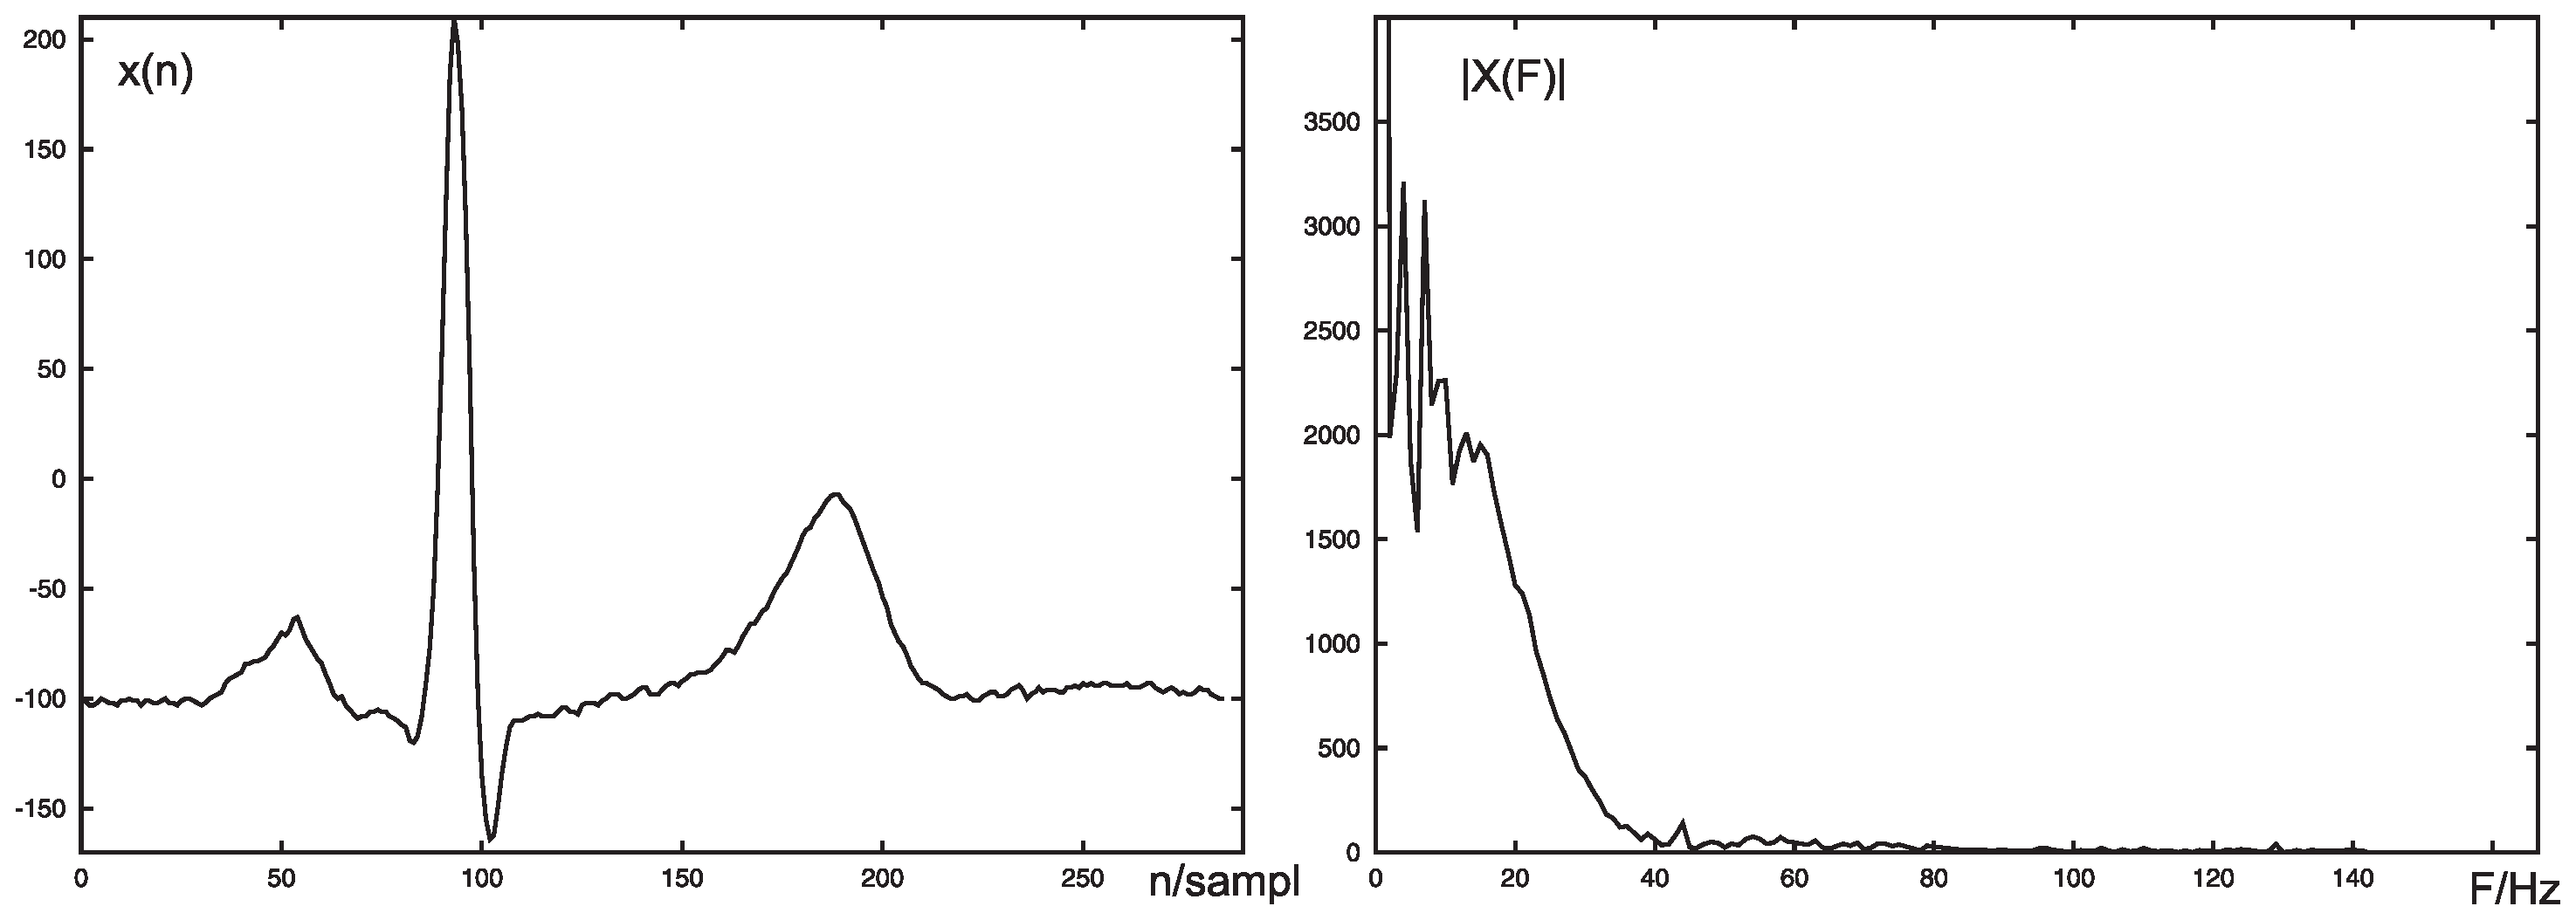
\includegraphics[width=\textwidth]{visualisation}%
\lthtmlpictureZ
\lthtmlcheckvsize\clearpage}

\stepcounter{subsection}
{\newpage\clearpage
\lthtmlinlinemathA{tex2html_wrap_inline2061}%
$|X(F)|$%
\lthtmlindisplaymathZ
\lthtmlcheckvsize\clearpage}

{\newpage\clearpage
\lthtmlinlinemathA{tex2html_wrap_inline2063}%
$\arg(X(F))$%
\lthtmlindisplaymathZ
\lthtmlcheckvsize\clearpage}

\stepcounter{section}
\stepcounter{subsection}
{\newpage\clearpage
\lthtmlpictureA{tex2html_wrap6221}%
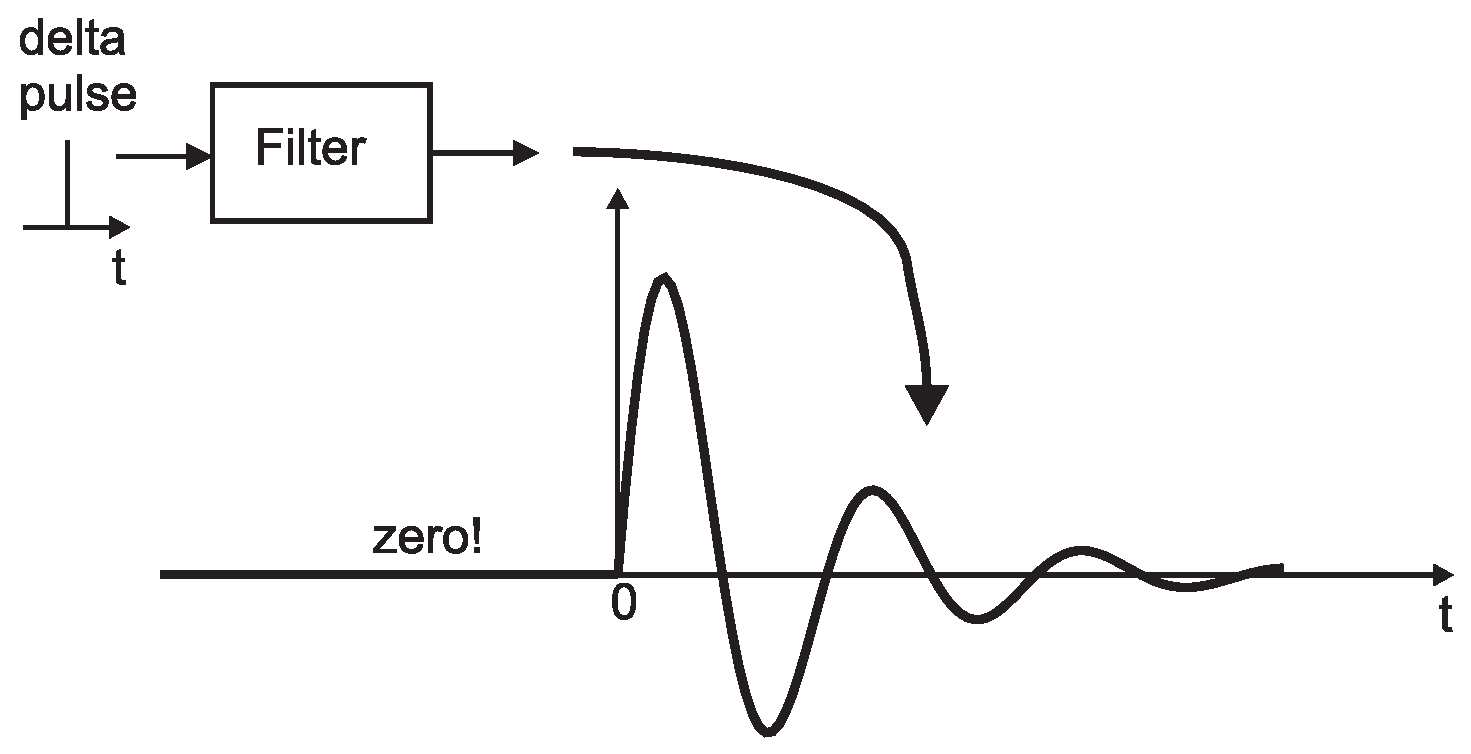
\includegraphics[width=0.75\textwidth]{causality}%
\lthtmlpictureZ
\lthtmlcheckvsize\clearpage}

\stepcounter{subsection}
{\newpage\clearpage
\lthtmlpictureA{tex2html_wrap6229}%
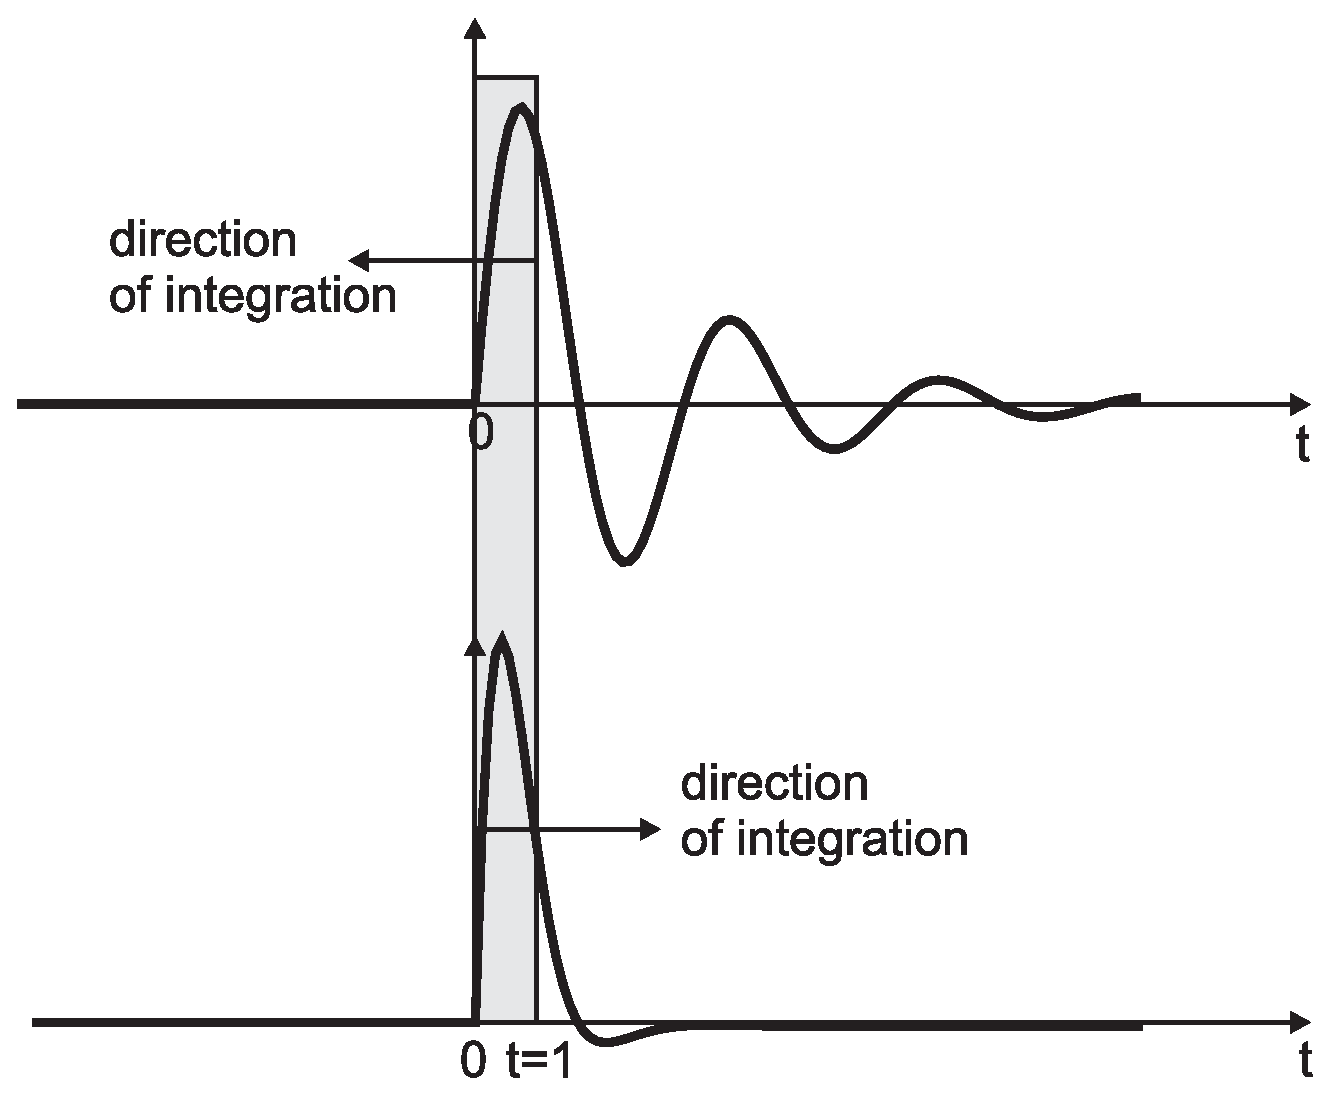
\includegraphics[width=0.75\textwidth]{convol}%
\lthtmlpictureZ
\lthtmlcheckvsize\clearpage}

\stepcounter{subsection}
{\newpage\clearpage
\lthtmlinlinemathA{tex2html_wrap_indisplay6237}%
$\displaystyle y(t)$%
\lthtmlindisplaymathZ
\lthtmlcheckvsize\clearpage}

{\newpage\clearpage
\lthtmlinlinemathA{tex2html_wrap_indisplay6239}%
$\displaystyle h(t) * x(t) = \int_{-\infty}^{\infty} h(t - \tau) x(\tau) d\tau$%
\lthtmlindisplaymathZ
\lthtmlcheckvsize\clearpage}

{\newpage\clearpage
\lthtmlinlinemathA{tex2html_wrap_indisplay6240}%
$\displaystyle y(n)$%
\lthtmlindisplaymathZ
\lthtmlcheckvsize\clearpage}

{\newpage\clearpage
\lthtmlinlinemathA{tex2html_wrap_indisplay6242}%
$\displaystyle h(n) * x(n) = \sum_{n = -\infty}^\infty h(n) x(m - n)$%
\lthtmlindisplaymathZ
\lthtmlcheckvsize\clearpage}

{\newpage\clearpage
\lthtmlinlinemathA{tex2html_wrap_inline2075}%
$h$%
\lthtmlindisplaymathZ
\lthtmlcheckvsize\clearpage}

{\newpage\clearpage
\lthtmlinlinemathA{tex2html_wrap_inline2079}%
$h(0)$%
\lthtmlindisplaymathZ
\lthtmlcheckvsize\clearpage}

{\newpage\clearpage
\lthtmlinlinemathA{tex2html_wrap_inline2081}%
$x(0)$%
\lthtmlindisplaymathZ
\lthtmlcheckvsize\clearpage}

{\newpage\clearpage
\lthtmlinlinemathA{tex2html_wrap_inline2085}%
$t>0$%
\lthtmlindisplaymathZ
\lthtmlcheckvsize\clearpage}

{\newpage\clearpage
\lthtmlinlinemathA{tex2html_wrap_inline2089}%
$x(t)=\delta(t)$%
\lthtmlindisplaymathZ
\lthtmlcheckvsize\clearpage}

{\newpage\clearpage
\lthtmlinlinemathA{tex2html_wrap_indisplay6252}%
$\displaystyle y(t) = \int_{-\infty}^{\infty} h(t - \tau) \delta(\tau) d\tau = h(t)
$%
\lthtmlindisplaymathZ
\lthtmlcheckvsize\clearpage}

{\newpage\clearpage
\lthtmlinlinemathA{tex2html_wrap_inline2091}%
$h(t)$%
\lthtmlindisplaymathZ
\lthtmlcheckvsize\clearpage}

\stepcounter{subsection}
{\newpage\clearpage
\lthtmlinlinemathA{tex2html_wrap_inline2093}%
$-\infty < t < +\infty$%
\lthtmlindisplaymathZ
\lthtmlcheckvsize\clearpage}

{\newpage\clearpage
\lthtmlinlinemathA{tex2html_wrap_indisplay6257}%
$\displaystyle {\mathrm{\bf L\!T}({h(t)})} = H(s) = \int_{0}^{\infty} h(t) e^{-st} dt
$%
\lthtmlindisplaymathZ
\lthtmlcheckvsize\clearpage}

{\newpage\clearpage
\lthtmlinlinemathA{tex2html_wrap_indisplay6259}%
$\displaystyle \int f(\tau) d\tau \Leftrightarrow \frac{1}{s} F(s)
$%
\lthtmlindisplaymathZ
\lthtmlcheckvsize\clearpage}

{\newpage\clearpage
\lthtmlinlinemathA{tex2html_wrap_indisplay6261}%
$\displaystyle \frac{d}{dt} f(t) \Leftrightarrow s F(s) 
$%
\lthtmlindisplaymathZ
\lthtmlcheckvsize\clearpage}

{\newpage\clearpage
\lthtmlinlinemathA{tex2html_wrap_indisplay6263}%
$\displaystyle f(t - T) \Leftrightarrow e^{-Ts} F(s)
$%
\lthtmlindisplaymathZ
\lthtmlcheckvsize\clearpage}

{\newpage\clearpage
\lthtmlinlinemathA{tex2html_wrap_indisplay6265}%
$\displaystyle {\mathrm{\bf L\!T}({h(t - T)})}$%
\lthtmlindisplaymathZ
\lthtmlcheckvsize\clearpage}

{\newpage\clearpage
\lthtmlinlinemathA{tex2html_wrap_indisplay6267}%
$\displaystyle \int_{0}^{\infty} h\underbrace{(t - T)}_{causal} e^{-st} dt$%
\lthtmlindisplaymathZ
\lthtmlcheckvsize\clearpage}

{\newpage\clearpage
\lthtmlinlinemathA{tex2html_wrap_indisplay6269}%
$\displaystyle \int_{0}^{\infty} h(t) e^{-s(t + T)} dt$%
\lthtmlindisplaymathZ
\lthtmlcheckvsize\clearpage}

{\newpage\clearpage
\lthtmlinlinemathA{tex2html_wrap_indisplay6271}%
$\displaystyle \int_{0}^{\infty} h(t) e^{-st} e^{-sT} dt$%
\lthtmlindisplaymathZ
\lthtmlcheckvsize\clearpage}

{\newpage\clearpage
\lthtmlinlinemathA{tex2html_wrap_indisplay6273}%
$\displaystyle e^{-sT} \underbrace{\int_{0}^{\infty} h(t) e^{-st} dt}_{H(s)}$%
\lthtmlindisplaymathZ
\lthtmlcheckvsize\clearpage}

{\newpage\clearpage
\lthtmlinlinemathA{tex2html_wrap_indisplay6275}%
$\displaystyle e^{-sT} H(s)$%
\lthtmlindisplaymathZ
\lthtmlcheckvsize\clearpage}

{\newpage\clearpage
\lthtmlinlinemathA{tex2html_wrap_indisplay6277}%
$\displaystyle f(t) * g(t) \Leftrightarrow F(s) G(s)
$%
\lthtmlindisplaymathZ
\lthtmlcheckvsize\clearpage}

{\newpage\clearpage
\lthtmlpictureA{tex2html_wrap6278}%
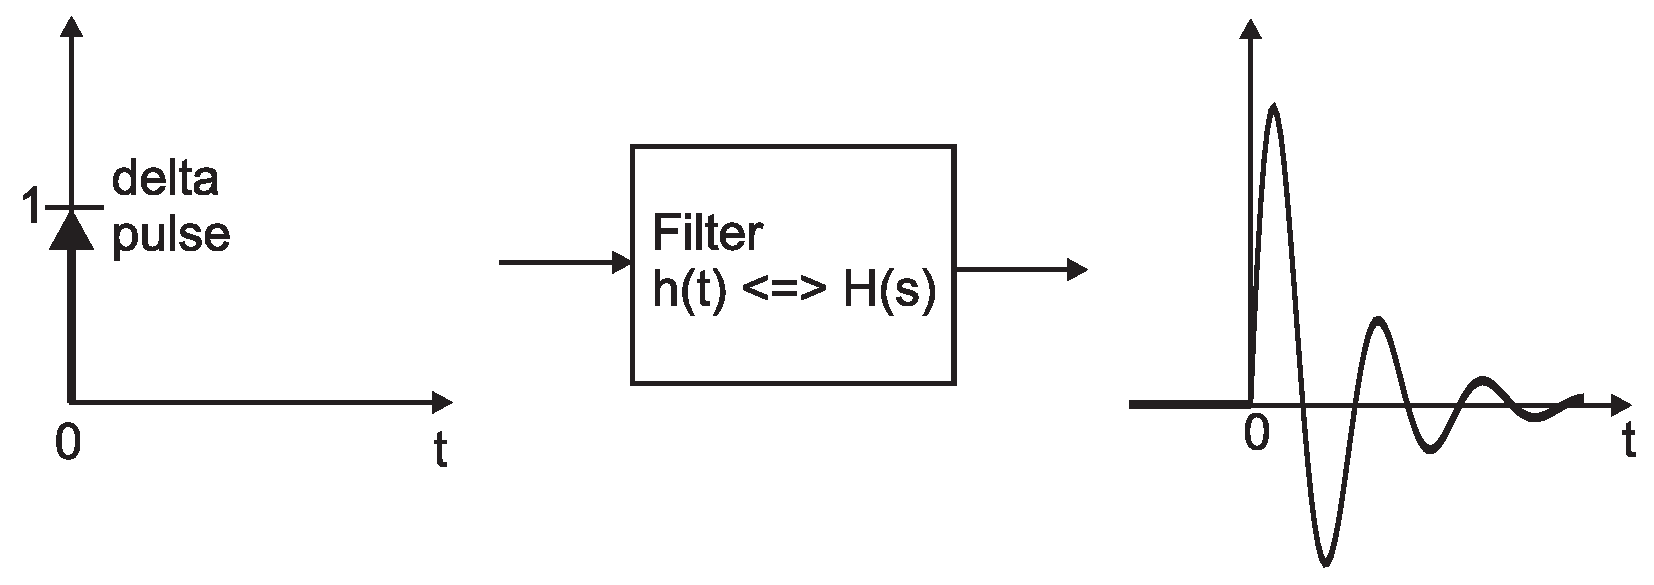
\includegraphics[width=0.75\textwidth]{filter}%
\lthtmlpictureZ
\lthtmlcheckvsize\clearpage}

\stepcounter{subsection}
{\newpage\clearpage
\lthtmlinlinemathA{tex2html_wrap_indisplay6284}%
$\displaystyle g(t) = h(t) * x(t) \Leftrightarrow Y(s) = H(s) \cdot X(s)
$%
\lthtmlindisplaymathZ
\lthtmlcheckvsize\clearpage}

\stepcounter{subsubsection}
{\newpage\clearpage
\lthtmlinlinemathA{tex2html_wrap_indisplay6289}%
$\displaystyle \delta(t) \qquad \leftarrow \mbox{delta pulse}$%
\lthtmlindisplaymathZ
\lthtmlcheckvsize\clearpage}

{\newpage\clearpage
\lthtmlinlinemathA{tex2html_wrap_indisplay6290}%
$\displaystyle h(t)$%
\lthtmlindisplaymathZ
\lthtmlcheckvsize\clearpage}

{\newpage\clearpage
\lthtmlinlinemathA{tex2html_wrap_indisplay6292}%
$\displaystyle y(t) \qquad \leftarrow \mbox{impulse response}$%
\lthtmlindisplaymathZ
\lthtmlcheckvsize\clearpage}

{\newpage\clearpage
\lthtmlinlinemathA{tex2html_wrap_inline2097}%
$j\omega$%
\lthtmlindisplaymathZ
\lthtmlcheckvsize\clearpage}

{\newpage\clearpage
\lthtmlinlinemathA{tex2html_wrap_indisplay6296}%
$\displaystyle |H(i \omega)|
$%
\lthtmlindisplaymathZ
\lthtmlcheckvsize\clearpage}

{\newpage\clearpage
\lthtmlinlinemathA{tex2html_wrap_inline2099}%
$H(j\omega)$%
\lthtmlindisplaymathZ
\lthtmlcheckvsize\clearpage}

{\newpage\clearpage
\lthtmlinlinemathA{tex2html_wrap_indisplay6299}%
$\displaystyle \phi = \arg\left(H(i \omega) \right)
$%
\lthtmlindisplaymathZ
\lthtmlcheckvsize\clearpage}

{\newpage\clearpage
\lthtmlinlinemathA{tex2html_wrap_indisplay6301}%
$\displaystyle \tau_{\omega} = \frac{d \phi (\omega)}{d\omega}
$%
\lthtmlindisplaymathZ
\lthtmlcheckvsize\clearpage}

{\newpage\clearpage
\lthtmlinlinemathA{tex2html_wrap_inline2101}%
$\omega$%
\lthtmlindisplaymathZ
\lthtmlcheckvsize\clearpage}

\stepcounter{subsection}
{\newpage\clearpage
\lthtmlinlinemathA{tex2html_wrap_indisplay6305}%
$\displaystyle x(t) = \sum_{n = 0}^{\infty} x(n) \delta(t - nT) \qquad \mbox{Sampled signal} 
$%
\lthtmlindisplaymathZ
\lthtmlcheckvsize\clearpage}

{\newpage\clearpage
\lthtmlinlinemathA{tex2html_wrap_indisplay6307}%
$\displaystyle X(s)$%
\lthtmlindisplaymathZ
\lthtmlcheckvsize\clearpage}

{\newpage\clearpage
\lthtmlinlinemathA{tex2html_wrap_indisplay6309}%
$\displaystyle \sum_{n = 0}^{\infty} x(n) e^{-snT}$%
\lthtmlindisplaymathZ
\lthtmlcheckvsize\clearpage}

{\newpage\clearpage
\lthtmlinlinemathA{tex2html_wrap_indisplay6311}%
$\displaystyle \int_{0}^{\infty} x(n) e^{-st} dt$%
\lthtmlindisplaymathZ
\lthtmlcheckvsize\clearpage}

{\newpage\clearpage
\lthtmlinlinemathA{tex2html_wrap_indisplay6313}%
$\displaystyle \sum_{n = 0}^{\infty} x(n) \underbrace{(e^{-sT})^{n}}_{z^{-1} = e^{-sT}}$%
\lthtmlindisplaymathZ
\lthtmlcheckvsize\clearpage}

{\newpage\clearpage
\lthtmlinlinemathA{tex2html_wrap_indisplay6315}%
$\displaystyle \sum_{n = 0}^{\infty} x(n) (z^{-1})^{n} \qquad \mbox{z-transform}$%
\lthtmlindisplaymathZ
\lthtmlcheckvsize\clearpage}

{\newpage\clearpage
\lthtmlinlinemathA{tex2html_wrap_inline2103}%
$e^{-sT} = z^{-1}$%
\lthtmlindisplaymathZ
\lthtmlcheckvsize\clearpage}

{\newpage\clearpage
\lthtmlpictureA{tex2html_wrap6317}%
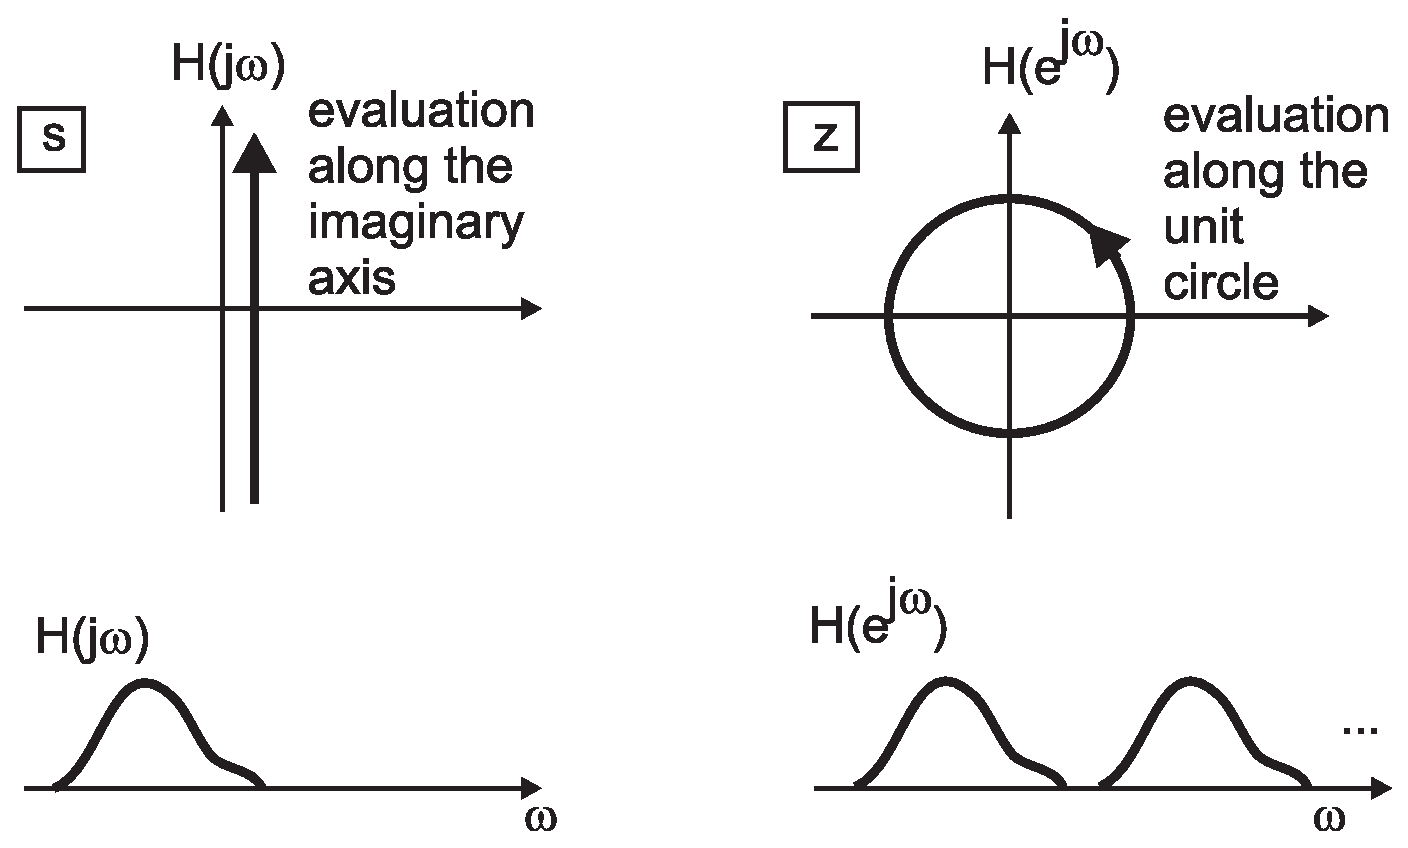
\includegraphics[width=0.75\textwidth]{frequency_response}%
\lthtmlpictureZ
\lthtmlcheckvsize\clearpage}

\stepcounter{subsection}
{\newpage\clearpage
\lthtmlinlinemathA{tex2html_wrap_inline2105}%
$H(s)$%
\lthtmlindisplaymathZ
\lthtmlcheckvsize\clearpage}

{\newpage\clearpage
\lthtmlinlinemathA{tex2html_wrap_inline2107}%
$s=j \omega$%
\lthtmlindisplaymathZ
\lthtmlcheckvsize\clearpage}

{\newpage\clearpage
\lthtmlinlinemathA{tex2html_wrap_inline2109}%
$s$%
\lthtmlindisplaymathZ
\lthtmlcheckvsize\clearpage}

{\newpage\clearpage
\lthtmlinlinemathA{tex2html_wrap_inline2111}%
$z$%
\lthtmlindisplaymathZ
\lthtmlcheckvsize\clearpage}

{\newpage\clearpage
\lthtmlinlinemathA{tex2html_wrap_inline2113}%
$z^{-1} = e^{-sT}$%
\lthtmlindisplaymathZ
\lthtmlcheckvsize\clearpage}

{\newpage\clearpage
\lthtmlinlinemathA{tex2html_wrap_indisplay6328}%
$\displaystyle z = e^{sT}
$%
\lthtmlindisplaymathZ
\lthtmlcheckvsize\clearpage}

{\newpage\clearpage
\lthtmlinlinemathA{tex2html_wrap_inline2117}%
$z = e^{j \omega}$%
\lthtmlindisplaymathZ
\lthtmlcheckvsize\clearpage}

{\newpage\clearpage
\lthtmlinlinemathA{tex2html_wrap_indisplay6332}%
$\displaystyle H(e^{j \omega})
$%
\lthtmlindisplaymathZ
\lthtmlcheckvsize\clearpage}

{\newpage\clearpage
\lthtmlinlinemathA{tex2html_wrap_indisplay6334}%
$\displaystyle |H(e^{i \omega})|
$%
\lthtmlindisplaymathZ
\lthtmlcheckvsize\clearpage}

{\newpage\clearpage
\lthtmlinlinemathA{tex2html_wrap_indisplay6336}%
$\displaystyle \arg H(e^{i \omega})
$%
\lthtmlindisplaymathZ
\lthtmlcheckvsize\clearpage}

\stepcounter{subsection}
{\newpage\clearpage
\lthtmlinlinemathA{tex2html_wrap_indisplay6340}%
$\displaystyle
h(t)=\sum_{n=0}^\infty h(nT) \delta(t-nT)
$%
\lthtmlindisplaymathZ
\lthtmlcheckvsize\clearpage}

{\newpage\clearpage
\lthtmlinlinemathA{tex2html_wrap_indisplay6342}%
$\displaystyle
H(s)=\sum_{n=0}^\infty h(nT) {\underbrace{{\left(e^{-sT}\right)}}_
                                           {z^{-1}}}^n
$%
\lthtmlindisplaymathZ
\lthtmlcheckvsize\clearpage}

{\newpage\clearpage
\lthtmlinlinemathA{tex2html_wrap_inline2121}%
$e^{-sT}$%
\lthtmlindisplaymathZ
\lthtmlcheckvsize\clearpage}

{\newpage\clearpage
\lthtmlinlinemathA{tex2html_wrap_inline2123}%
$z^{-n}$%
\lthtmlindisplaymathZ
\lthtmlcheckvsize\clearpage}

{\newpage\clearpage
\lthtmlinlinemathA{tex2html_wrap_indisplay6347}%
$\displaystyle H(z)=\sum_{n=0}^\infty h(nT) {(z^{-1})}^n
$%
\lthtmlindisplaymathZ
\lthtmlcheckvsize\clearpage}

{\newpage\clearpage
\lthtmlinlinemathA{tex2html_wrap_inline2129}%
$X(z)$%
\lthtmlindisplaymathZ
\lthtmlcheckvsize\clearpage}

{\newpage\clearpage
\lthtmlinlinemathA{tex2html_wrap_inline2131}%
$H(z)$%
\lthtmlindisplaymathZ
\lthtmlcheckvsize\clearpage}

{\newpage\clearpage
\lthtmlinlinemathA{tex2html_wrap_indisplay6352}%
$\displaystyle H(z)X(z)=\underbrace{\sum_{n=0}^\infty h(nT) z^{-n}}_{H(z)} X(z)
$%
\lthtmlindisplaymathZ
\lthtmlcheckvsize\clearpage}

{\newpage\clearpage
\lthtmlinlinemathA{tex2html_wrap_inline2135}%
$h(nT)$%
\lthtmlindisplaymathZ
\lthtmlcheckvsize\clearpage}

{\newpage\clearpage
\lthtmlinlinemathA{tex2html_wrap_inline2137}%
$100$%
\lthtmlindisplaymathZ
\lthtmlcheckvsize\clearpage}

{\newpage\clearpage
\lthtmlinlinemathA{tex2html_wrap_inline2143}%
$N=100$%
\lthtmlindisplaymathZ
\lthtmlcheckvsize\clearpage}

{\newpage\clearpage
\lthtmlinlinemathA{tex2html_wrap_indisplay6360}%
$\displaystyle
H(z)X(z)=\underbrace{\sum_{n=0}^N h(nT) z^{-n}}_{H(z)} X(z)
$%
\lthtmlindisplaymathZ
\lthtmlcheckvsize\clearpage}

{\newpage\clearpage
\lthtmlpictureA{tex2html_wrap6361}%
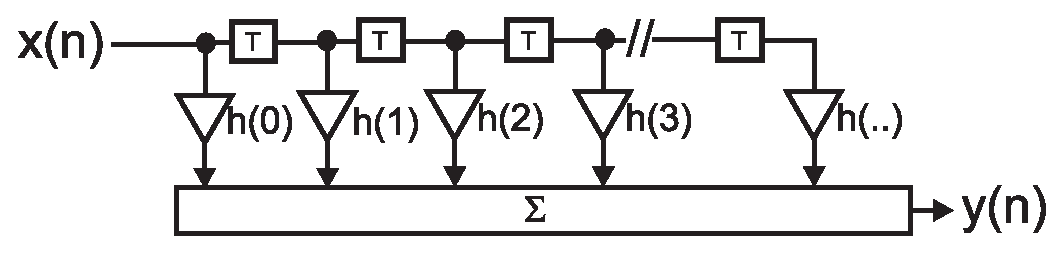
\includegraphics[width=\linewidth]{fir_digital}%
\lthtmlpictureZ
\lthtmlcheckvsize\clearpage}

{\newpage\clearpage
\lthtmlinlinemathA{tex2html_wrap_inline2151}%
$h(n)$%
\lthtmlindisplaymathZ
\lthtmlcheckvsize\clearpage}

{\newpage\clearpage
\lthtmlinlinemathA{tex2html_wrap_indisplay6371}%
$\displaystyle H(z)X(z)$%
\lthtmlindisplaymathZ
\lthtmlcheckvsize\clearpage}

{\newpage\clearpage
\lthtmlinlinemathA{tex2html_wrap_indisplay6373}%
$\displaystyle \sum_{n=0}^N h_\textrm{\footnotesize {analogue}}(nT) z^{-n} \, X(z)$%
\lthtmlindisplaymathZ
\lthtmlcheckvsize\clearpage}

{\newpage\clearpage
\lthtmlinlinemathA{tex2html_wrap_indisplay6376}%
$\displaystyle \sum_{n=0}^N h_\textrm{\footnotesize {digital}}(n) z^{-n} \, X(z)$%
\lthtmlindisplaymathZ
\lthtmlcheckvsize\clearpage}

{\newpage\clearpage
\lthtmlinlinemathA{tex2html_wrap_indisplay6378}%
$\displaystyle \sum_{n=0}^N h_(n) z^{-n} \, X(z)$%
\lthtmlindisplaymathZ
\lthtmlcheckvsize\clearpage}

{\newpage\clearpage
\lthtmlinlinemathA{tex2html_wrap_inline2155}%
$0$%
\lthtmlindisplaymathZ
\lthtmlcheckvsize\clearpage}

\stepcounter{subsubsection}
\stepcounter{subsubsection}
{\newpage\clearpage
\lthtmlpictureA{tex2html_wrap6384}%
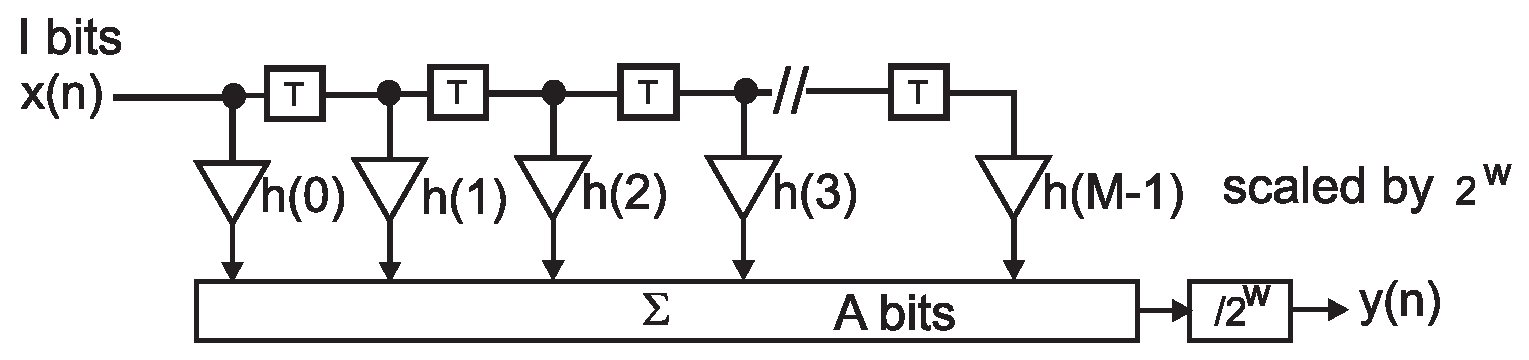
\includegraphics[width=\linewidth]{fir_fixed}%
\lthtmlpictureZ
\lthtmlcheckvsize\clearpage}

\stepcounter{subsubsection}
{\newpage\clearpage
\lthtmlinlinemathA{tex2html_wrap_inline2169}%
$-0.75$%
\lthtmlindisplaymathZ
\lthtmlcheckvsize\clearpage}

{\newpage\clearpage
\lthtmlinlinemathA{tex2html_wrap_inline2171}%
$+0.75$%
\lthtmlindisplaymathZ
\lthtmlcheckvsize\clearpage}

{\newpage\clearpage
\lthtmlinlinemathA{tex2html_wrap_inline2173}%
$2^W, W=15$%
\lthtmlindisplaymathZ
\lthtmlcheckvsize\clearpage}

{\newpage\clearpage
\lthtmlinlinemathA{tex2html_wrap_inline2175}%
$2^W$%
\lthtmlindisplaymathZ
\lthtmlcheckvsize\clearpage}

{\newpage\clearpage
\lthtmlinlinemathA{tex2html_wrap_inline2177}%
$M$%
\lthtmlindisplaymathZ
\lthtmlcheckvsize\clearpage}

{\newpage\clearpage
\lthtmlinlinemathA{tex2html_wrap_inline2179}%
$\log_2 M$%
\lthtmlindisplaymathZ
\lthtmlcheckvsize\clearpage}

{\newpage\clearpage
\lthtmlinlinemathA{tex2html_wrap_indisplay6402}%
$\displaystyle A = I + W + \log_2 M
$%
\lthtmlindisplaymathZ
\lthtmlcheckvsize\clearpage}

{\newpage\clearpage
\lthtmlinlinemathA{tex2html_wrap_indisplay6405}%
$\displaystyle A = I + W
$%
\lthtmlindisplaymathZ
\lthtmlcheckvsize\clearpage}

{\newpage\clearpage
\lthtmlinlinemathA{tex2html_wrap_inline2183}%
$16$%
\lthtmlindisplaymathZ
\lthtmlcheckvsize\clearpage}

{\newpage\clearpage
\lthtmlinlinemathA{tex2html_wrap_inline2185}%
$32$%
\lthtmlindisplaymathZ
\lthtmlcheckvsize\clearpage}

\stepcounter{subsubsection}
{\newpage\clearpage
\lthtmlinlinemathA{tex2html_wrap_indisplay6410}%
$\displaystyle \tau_\omega={d\phi(\omega)\over d\omega}
$%
\lthtmlindisplaymathZ
\lthtmlcheckvsize\clearpage}

{\newpage\clearpage
\lthtmlinlinemathA{tex2html_wrap_inline2187}%
$\tau_\omega$%
\lthtmlindisplaymathZ
\lthtmlcheckvsize\clearpage}

{\newpage\clearpage
\lthtmlinlinemathA{tex2html_wrap_indisplay6415}%
$\displaystyle H(e^{i\omega})=B(\omega)e^{-i\omega\tau+i\phi}
$%
\lthtmlindisplaymathZ
\lthtmlcheckvsize\clearpage}

{\newpage\clearpage
\lthtmlinlinemathA{tex2html_wrap_inline2193}%
$B(\omega)$%
\lthtmlindisplaymathZ
\lthtmlcheckvsize\clearpage}

{\newpage\clearpage
\lthtmlinlinemathA{tex2html_wrap_inline2195}%
$\omega\tau+\phi$%
\lthtmlindisplaymathZ
\lthtmlcheckvsize\clearpage}

{\newpage\clearpage
\lthtmlinlinemathA{tex2html_wrap_indisplay6420}%
$\displaystyle h(n)=\frac{1}{2\pi}\int_{-\infty}^{+\infty} H(e^{i\omega})
e^{i\omega n}d \omega
$%
\lthtmlindisplaymathZ
\lthtmlcheckvsize\clearpage}

{\newpage\clearpage
\lthtmlinlinemathA{tex2html_wrap_indisplay6422}%
$\displaystyle h(n+\tau)=\frac{1}{2\pi}e^{i\phi}b(n)
$%
\lthtmlindisplaymathZ
\lthtmlcheckvsize\clearpage}

{\newpage\clearpage
\lthtmlinlinemathA{tex2html_wrap_inline2199}%
$b(n)$%
\lthtmlindisplaymathZ
\lthtmlcheckvsize\clearpage}

{\newpage\clearpage
\lthtmlinlinemathA{tex2html_wrap_inline2207}%
$b(n)=b^*(-n)$%
\lthtmlindisplaymathZ
\lthtmlcheckvsize\clearpage}

{\newpage\clearpage
\lthtmlinlinemathA{tex2html_wrap_indisplay6429}%
$\displaystyle h(n+\tau)=\frac{1}{2\pi}e^{i\phi}b^*(-n)
$%
\lthtmlindisplaymathZ
\lthtmlcheckvsize\clearpage}

{\newpage\clearpage
\lthtmlinlinemathA{tex2html_wrap_inline2209}%
$b$%
\lthtmlindisplaymathZ
\lthtmlcheckvsize\clearpage}

{\newpage\clearpage
\lthtmlinlinemathA{tex2html_wrap_indisplay6432}%
$\displaystyle h(n+\tau)=e^{2i\phi} n^*(-n+\tau)
$%
\lthtmlindisplaymathZ
\lthtmlcheckvsize\clearpage}

{\newpage\clearpage
\lthtmlinlinemathA{tex2html_wrap_inline2211}%
$\tau$%
\lthtmlindisplaymathZ
\lthtmlcheckvsize\clearpage}

{\newpage\clearpage
\lthtmlinlinemathA{tex2html_wrap_inline2215}%
$n<0$%
\lthtmlindisplaymathZ
\lthtmlcheckvsize\clearpage}

{\newpage\clearpage
\lthtmlinlinemathA{tex2html_wrap_inline2219}%
$\tau=M/2$%
\lthtmlindisplaymathZ
\lthtmlcheckvsize\clearpage}

{\newpage\clearpage
\lthtmlinlinemathA{tex2html_wrap_inline2221}%
$e^{2i\phi}$%
\lthtmlindisplaymathZ
\lthtmlcheckvsize\clearpage}

{\newpage\clearpage
\lthtmlinlinemathA{tex2html_wrap_inline2223}%
$\phi$%
\lthtmlindisplaymathZ
\lthtmlcheckvsize\clearpage}

{\newpage\clearpage
\lthtmlinlinemathA{tex2html_wrap_indisplay6441}%
$\displaystyle h(n+M/2)=(-1)^k h(-n+M/2)
$%
\lthtmlindisplaymathZ
\lthtmlcheckvsize\clearpage}

{\newpage\clearpage
\lthtmlinlinemathA{tex2html_wrap_inline2225}%
$k=0$%
\lthtmlindisplaymathZ
\lthtmlcheckvsize\clearpage}

{\newpage\clearpage
\lthtmlpictureA{tex2html_wrap6445}%
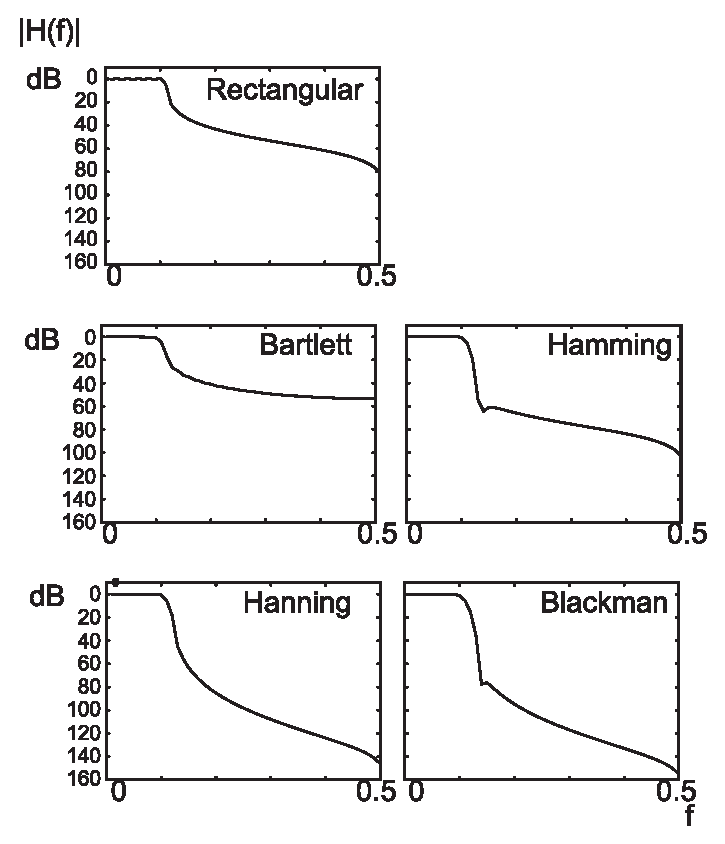
\includegraphics[width=\linewidth]{window_functions}%
\lthtmlpictureZ
\lthtmlcheckvsize\clearpage}

\stepcounter{subsubsection}
{\newpage\clearpage
\lthtmlinlinemathA{tex2html_wrap_inline2233}%
$M/2$%
\lthtmlindisplaymathZ
\lthtmlcheckvsize\clearpage}

{\newpage\clearpage
\lthtmlinlinemathA{tex2html_wrap_inline2235}%
$n>N$%
\lthtmlindisplaymathZ
\lthtmlcheckvsize\clearpage}

{\newpage\clearpage
\lthtmlinlinemathA{tex2html_wrap_indisplay6455}%
$\displaystyle
H(z)X(z)=\sum_{n=0}^N \underbrace{h(nT) w(nT)} z^{-n} X(z)
$%
\lthtmlindisplaymathZ
\lthtmlcheckvsize\clearpage}

{\newpage\clearpage
\lthtmlinlinemathA{tex2html_wrap_indisplay6457}%
$\displaystyle w(n) = \alpha - (1-\alpha) \cos\left(\frac{2\pi n}{M}\right)
$%
\lthtmlindisplaymathZ
\lthtmlcheckvsize\clearpage}

{\newpage\clearpage
\lthtmlinlinemathA{tex2html_wrap_inline2237}%
$\alpha = 0.54$%
\lthtmlindisplaymathZ
\lthtmlcheckvsize\clearpage}

{\newpage\clearpage
\lthtmlinlinemathA{tex2html_wrap_inline2239}%
$\alpha = 0.5$%
\lthtmlindisplaymathZ
\lthtmlcheckvsize\clearpage}

{\newpage\clearpage
\lthtmlinlinemathA{tex2html_wrap_indisplay6461}%
$\displaystyle w(n) = 0.42 + 0.5 \cos \left(\frac{2 \pi n}{M}\right) + 
0.08 \cos \left( \frac{4 \pi n}{M} \right) 
$%
\lthtmlindisplaymathZ
\lthtmlcheckvsize\clearpage}

{\newpage\clearpage
\lthtmlinlinemathA{tex2html_wrap_inline2241}%
$f_c=0.1$%
\lthtmlindisplaymathZ
\lthtmlcheckvsize\clearpage}

\stepcounter{subsubsection}
{\newpage\clearpage
\lthtmlinlinemathA{tex2html_wrap_inline2243}%
$50Hz$%
\lthtmlindisplaymathZ
\lthtmlcheckvsize\clearpage}

{\newpage\clearpage
\lthtmlinlinemathA{tex2html_wrap_inline2245}%
$1kHz$%
\lthtmlindisplaymathZ
\lthtmlcheckvsize\clearpage}

{\newpage\clearpage
\lthtmlinlinemathA{tex2html_wrap_inline2247}%
$N/2=50$%
\lthtmlindisplaymathZ
\lthtmlcheckvsize\clearpage}

{\newpage\clearpage
\lthtmlinlinemathA{tex2html_wrap_inline2249}%
$500Hz$%
\lthtmlindisplaymathZ
\lthtmlcheckvsize\clearpage}

{\newpage\clearpage
\lthtmlinlinemathA{tex2html_wrap_inline2253}%
$5$%
\lthtmlindisplaymathZ
\lthtmlcheckvsize\clearpage}

{\newpage\clearpage
\lthtmlinlinemathA{tex2html_wrap_inline2255}%
$50$%
\lthtmlindisplaymathZ
\lthtmlcheckvsize\clearpage}

\stepcounter{subsubsection}
{\newpage\clearpage
\lthtmlinlinemathA{tex2html_wrap_indisplay6473}%
$\displaystyle |H(e^{j\omega})| = \underbrace{B(e^{j\omega})}_{\mbox{real}}
$%
\lthtmlindisplaymathZ
\lthtmlcheckvsize\clearpage}

{\newpage\clearpage
\lthtmlinlinemathA{tex2html_wrap_indisplay6476}%
$\displaystyle |H(e^{j\omega})| =
\left\{
\begin{array}{ll}
1 & \mbox{for } |\omega| \leq \omega_{c} \\
0 & \mbox{for } \omega_c < |\omega| \leq \pi
\end{array}
\right.
$%
\lthtmlindisplaymathZ
\lthtmlcheckvsize\clearpage}

{\newpage\clearpage
\lthtmlinlinemathA{tex2html_wrap_indisplay6478}%
$\displaystyle h(n)$%
\lthtmlindisplaymathZ
\lthtmlcheckvsize\clearpage}

{\newpage\clearpage
\lthtmlinlinemathA{tex2html_wrap_indisplay6480}%
$\displaystyle \frac{1}{2 \pi} \int_{-\pi}^{\pi} H(e^{j \omega}) e^{j \omega n} d\omega$%
\lthtmlindisplaymathZ
\lthtmlcheckvsize\clearpage}

{\newpage\clearpage
\lthtmlinlinemathA{tex2html_wrap_indisplay6482}%
$\displaystyle \frac{1}{2 \pi} \int_{- \omega_{c}}^{+ \omega_{c}} e^{j \omega n} d\omega$%
\lthtmlindisplaymathZ
\lthtmlcheckvsize\clearpage}

{\newpage\clearpage
\lthtmlinlinemathA{tex2html_wrap_indisplay6484}%
$\displaystyle \frac{1}{2 \pi} \left[\frac{1}{jn} e^{j \omega n} \right]_{- \omega_{c}}^{+ \omega_{c}}$%
\lthtmlindisplaymathZ
\lthtmlcheckvsize\clearpage}

{\newpage\clearpage
\lthtmlinlinemathA{tex2html_wrap_indisplay6486}%
$\displaystyle \frac{1}{2 \pi jn} \left( e^{j \omega_{c} n} - e^{-j \omega_{c}n} \right)$%
\lthtmlindisplaymathZ
\lthtmlcheckvsize\clearpage}

{\newpage\clearpage
\lthtmlinlinemathA{tex2html_wrap_indisplay6488}%
$\displaystyle \sin z$%
\lthtmlindisplaymathZ
\lthtmlcheckvsize\clearpage}

{\newpage\clearpage
\lthtmlinlinemathA{tex2html_wrap_indisplay6490}%
$\displaystyle \frac{1}{2j} (e^{zj} - e^{-zj})$%
\lthtmlindisplaymathZ
\lthtmlcheckvsize\clearpage}

{\newpage\clearpage
\lthtmlinlinemathA{tex2html_wrap_indisplay6491}%
$\displaystyle \cos z$%
\lthtmlindisplaymathZ
\lthtmlcheckvsize\clearpage}

{\newpage\clearpage
\lthtmlinlinemathA{tex2html_wrap_indisplay6493}%
$\displaystyle \frac{1}{2} (e^{zj} + e^{-zj})$%
\lthtmlindisplaymathZ
\lthtmlcheckvsize\clearpage}

{\newpage\clearpage
\lthtmlinlinemathA{tex2html_wrap_indisplay6495}%
$\displaystyle h(n) = 
\left\{
\begin{array}{cc}
\frac{1}{\pi n} \sin \omega_{c}n & \mbox{for } n \neq 0 \\
\frac{\omega_{c}}{\pi} & \mbox{for }n = 0
\end{array}
\right.
$%
\lthtmlindisplaymathZ
\lthtmlcheckvsize\clearpage}

{\newpage\clearpage
\lthtmlinlinemathA{tex2html_wrap_inline2259}%
$\omega_c=2\pi f_c$%
\lthtmlindisplaymathZ
\lthtmlcheckvsize\clearpage}

{\newpage\clearpage
\lthtmlinlinemathA{tex2html_wrap_indisplay6498}%
$\displaystyle h(n) = 
\left\{
\begin{array}{ll}
\frac{\omega_c}{\pi} & \mbox{for $n=0$} \\
\frac{1}{\pi n} \sin(\omega_c n) & \mbox{for $n\neq 0$}
\end{array}
\right.
$%
\lthtmlindisplaymathZ
\lthtmlcheckvsize\clearpage}

{\newpage\clearpage
\lthtmlinlinemathA{tex2html_wrap_indisplay6501}%
$\displaystyle h(n)=
\left\{ 
\begin{array}{ll}
1-\frac{\omega_c}{\pi} & \mbox{for $n=0$} \\
-\frac{1}{\pi n} \sin(\omega_c n) & \mbox{for $n\neq 0$}
\end{array}
\right.
$%
\lthtmlindisplaymathZ
\lthtmlcheckvsize\clearpage}

{\newpage\clearpage
\lthtmlinlinemathA{tex2html_wrap_inline2271}%
$\omega_{1,2}=2\pi f_{1,2}$%
\lthtmlindisplaymathZ
\lthtmlcheckvsize\clearpage}

{\newpage\clearpage
\lthtmlinlinemathA{tex2html_wrap_indisplay6504}%
$\displaystyle h(n)=
\left\{ 
\begin{array}{ll}
\frac{\omega_2-\omega_1}{\pi} & \mbox{for $n=0$} \\
\frac{1}{\pi n}(\sin(\omega_2 n)-\sin(\omega_1 n)) & \mbox{for $n\neq 0$}
\end{array}
\right.
$%
\lthtmlindisplaymathZ
\lthtmlcheckvsize\clearpage}

{\newpage\clearpage
\lthtmlinlinemathA{tex2html_wrap_indisplay6507}%
$\displaystyle h(n)=
\left\{ 
\begin{array}{ll}
1-\frac{\omega_2-\omega_1}{\pi} & \mbox{for $n=0$} \\
\frac{1}{\pi n}(\sin(\omega_1 n)-\sin(\omega_2 n)) & \mbox{for $n\neq 0$}
\end{array}
\right.
$%
\lthtmlindisplaymathZ
\lthtmlcheckvsize\clearpage}

\stepcounter{subsubsection}
\stepcounter{subsubsection}
\stepcounter{subsection}
{\newpage\clearpage
\lthtmlinlinemathA{tex2html_wrap_indisplay6515}%
$\displaystyle e(t) = \int_{0}^{t} \underbrace{s(\tau)}_{\mbox{signal}} \underbrace{r(\tau)}_{\mbox{template}} d(\tau)
$%
\lthtmlindisplaymathZ
\lthtmlcheckvsize\clearpage}

{\newpage\clearpage
\lthtmlinlinemathA{tex2html_wrap_indisplay6517}%
$\displaystyle e(t) = \int_{0}^{\infty} s(\tau) h(t - \tau) d\tau 
$%
\lthtmlindisplaymathZ
\lthtmlcheckvsize\clearpage}

{\newpage\clearpage
\lthtmlinlinemathA{tex2html_wrap_inline2289}%
$h(t) : = r(T - \tau)$%
\lthtmlindisplaymathZ
\lthtmlcheckvsize\clearpage}

{\newpage\clearpage
\lthtmlinlinemathA{tex2html_wrap_inline2291}%
$0\ldots T$%
\lthtmlindisplaymathZ
\lthtmlcheckvsize\clearpage}

{\newpage\clearpage
\lthtmlinlinemathA{tex2html_wrap_indisplay6521}%
$\displaystyle e(t)$%
\lthtmlindisplaymathZ
\lthtmlcheckvsize\clearpage}

{\newpage\clearpage
\lthtmlinlinemathA{tex2html_wrap_indisplay6523}%
$\displaystyle \int_{0}^{T} s(\tau) r \left(T - (t - \tau)\right) d\tau$%
\lthtmlindisplaymathZ
\lthtmlcheckvsize\clearpage}

{\newpage\clearpage
\lthtmlinlinemathA{tex2html_wrap_indisplay6525}%
$\displaystyle \int_{0}^{T} s(\tau) r(T - t + \tau) d\tau$%
\lthtmlindisplaymathZ
\lthtmlcheckvsize\clearpage}

{\newpage\clearpage
\lthtmlinlinemathA{tex2html_wrap_inline2293}%
$t: = T$%
\lthtmlindisplaymathZ
\lthtmlcheckvsize\clearpage}

{\newpage\clearpage
\lthtmlinlinemathA{tex2html_wrap_indisplay6528}%
$\displaystyle e(T) = \int_{0}^{\infty} s(\tau) r (\tau) d\tau
$%
\lthtmlindisplaymathZ
\lthtmlcheckvsize\clearpage}

{\newpage\clearpage
\lthtmlinlinemathA{tex2html_wrap_indisplay6530}%
$\displaystyle \underbrace{h(t) : = r(T - t)}_{ matched \quad  filter!} 
$%
\lthtmlindisplaymathZ
\lthtmlcheckvsize\clearpage}

{\newpage\clearpage
\lthtmlpictureA{tex2html_wrap6533}%
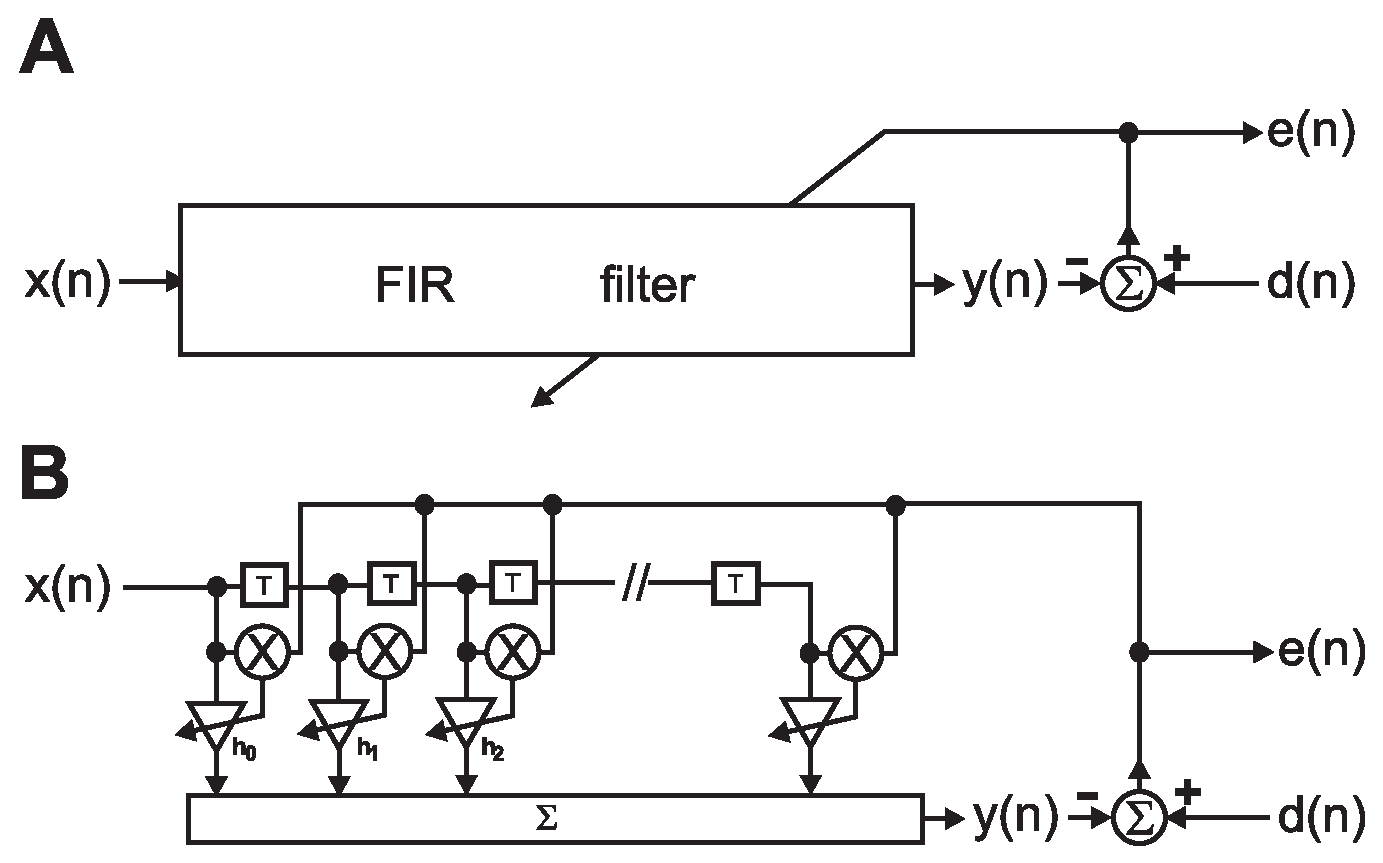
\includegraphics[width=\linewidth]{fir_lms}%
\lthtmlpictureZ
\lthtmlcheckvsize\clearpage}

\stepcounter{subsection}
{\newpage\clearpage
\lthtmlinlinemathA{tex2html_wrap_inline2299}%
$e(n)$%
\lthtmlindisplaymathZ
\lthtmlcheckvsize\clearpage}

{\newpage\clearpage
\lthtmlinlinemathA{tex2html_wrap_inline2301}%
$y(n)$%
\lthtmlindisplaymathZ
\lthtmlcheckvsize\clearpage}

{\newpage\clearpage
\lthtmlinlinemathA{tex2html_wrap_inline2303}%
$d(n)$%
\lthtmlindisplaymathZ
\lthtmlcheckvsize\clearpage}

{\newpage\clearpage
\lthtmlinlinemathA{tex2html_wrap_indisplay6542}%
$\displaystyle e(n) = d(n) - y(n)
$%
\lthtmlindisplaymathZ
\lthtmlcheckvsize\clearpage}

{\newpage\clearpage
\lthtmlinlinemathA{tex2html_wrap_indisplay6544}%
$\displaystyle \Delta h_j = - \mu \frac{\partial \frac{1}{2}e(n)^2}{\partial h_j}
$%
\lthtmlindisplaymathZ
\lthtmlcheckvsize\clearpage}

{\newpage\clearpage
\lthtmlinlinemathA{tex2html_wrap_inline2305}%
$h_j$%
\lthtmlindisplaymathZ
\lthtmlcheckvsize\clearpage}

{\newpage\clearpage
\lthtmlinlinemathA{tex2html_wrap_inline2307}%
$e(n), d(n)$%
\lthtmlindisplaymathZ
\lthtmlcheckvsize\clearpage}

{\newpage\clearpage
\lthtmlinlinemathA{tex2html_wrap_inline2313}%
$\epsilon$%
\lthtmlindisplaymathZ
\lthtmlcheckvsize\clearpage}

{\newpage\clearpage
\lthtmlinlinemathA{tex2html_wrap_inline2315}%
$h_j := h_j + \epsilon$%
\lthtmlindisplaymathZ
\lthtmlcheckvsize\clearpage}

{\newpage\clearpage
\lthtmlinlinemathA{tex2html_wrap_inline2317}%
$\frac{1}{2}e(n)^2$%
\lthtmlindisplaymathZ
\lthtmlcheckvsize\clearpage}

{\newpage\clearpage
\lthtmlinlinemathA{tex2html_wrap_indisplay6558}%
$\displaystyle \Delta h_j$%
\lthtmlindisplaymathZ
\lthtmlcheckvsize\clearpage}

{\newpage\clearpage
\lthtmlinlinemathA{tex2html_wrap_indisplay6560}%
$\displaystyle - \mu \frac{\partial \frac{1}{2}\left(d(n)-y(n)\right)^2}{\partial h_j}$%
\lthtmlindisplaymathZ
\lthtmlcheckvsize\clearpage}

{\newpage\clearpage
\lthtmlinlinemathA{tex2html_wrap_indisplay6562}%
$\displaystyle - \mu \frac{\partial \frac{1}{2}\left(d(n)-\sum_j x_j(n) h_j(n)\right)^2}{\partial h_j}$%
\lthtmlindisplaymathZ
\lthtmlcheckvsize\clearpage}

{\newpage\clearpage
\lthtmlinlinemathA{tex2html_wrap_indisplay6564}%
$\displaystyle \mu \left(d(n)-y(n)\right) x_j(n)$%
\lthtmlindisplaymathZ
\lthtmlcheckvsize\clearpage}

{\newpage\clearpage
\lthtmlinlinemathA{tex2html_wrap_indisplay6566}%
$\displaystyle \mu e(n) x_j(n)$%
\lthtmlindisplaymathZ
\lthtmlcheckvsize\clearpage}

{\newpage\clearpage
\lthtmlinlinemathA{tex2html_wrap_inline2329}%
$\mu$%
\lthtmlindisplaymathZ
\lthtmlcheckvsize\clearpage}

{\newpage\clearpage
\lthtmlinlinemathA{tex2html_wrap_inline2331}%
$x_j(n)$%
\lthtmlindisplaymathZ
\lthtmlcheckvsize\clearpage}

\stepcounter{subsection}
\stepcounter{subsubsection}
{\newpage\clearpage
\lthtmlinlinemathA{tex2html_wrap_indisplay6576}%
$\displaystyle h(t)=e^{-bt}
$%
\lthtmlindisplaymathZ
\lthtmlcheckvsize\clearpage}

{\newpage\clearpage
\lthtmlinlinemathA{tex2html_wrap_indisplay6578}%
$\displaystyle H(s)=\frac{1}{s+b}
$%
\lthtmlindisplaymathZ
\lthtmlcheckvsize\clearpage}

{\newpage\clearpage
\lthtmlinlinemathA{tex2html_wrap_indisplay6580}%
$\displaystyle h(t)=\sum_{n=0}^\infty e^{-bnT} \cdot \delta(t-nT)
$%
\lthtmlindisplaymathZ
\lthtmlcheckvsize\clearpage}

{\newpage\clearpage
\lthtmlinlinemathA{tex2html_wrap_indisplay6582}%
$\displaystyle H(s) = \sum_{n=0}^\infty e^{-bnT} \underbrace{e^{-nsT}}_{{z^{-1}}^n}
$%
\lthtmlindisplaymathZ
\lthtmlcheckvsize\clearpage}

{\newpage\clearpage
\lthtmlinlinemathA{tex2html_wrap_indisplay6584}%
$\displaystyle H(z)$%
\lthtmlindisplaymathZ
\lthtmlcheckvsize\clearpage}

{\newpage\clearpage
\lthtmlinlinemathA{tex2html_wrap_indisplay6586}%
$\displaystyle \sum_{n=0}^\infty e^{-bnT} z^{-n}$%
\lthtmlindisplaymathZ
\lthtmlcheckvsize\clearpage}

{\newpage\clearpage
\lthtmlinlinemathA{tex2html_wrap_indisplay6588}%
$\displaystyle \sum_{n=0}^\infty {\left(e^{-bT} z^{-1}\right)}^n$%
\lthtmlindisplaymathZ
\lthtmlcheckvsize\clearpage}

{\newpage\clearpage
\lthtmlinlinemathA{tex2html_wrap_indisplay6590}%
$\displaystyle {1\over 1-e^{-bT} z^{-1}}$%
\lthtmlindisplaymathZ
\lthtmlcheckvsize\clearpage}

{\newpage\clearpage
\lthtmlinlinemathA{tex2html_wrap_indisplay6594}%
$\displaystyle H(s)=\frac{1}{s+b} \qquad\Leftrightarrow\qquad
H(z)=\frac{1}{1-e^{-bT} z^{-1}}
$%
\lthtmlindisplaymathZ
\lthtmlcheckvsize\clearpage}

{\newpage\clearpage
\lthtmlinlinemathA{tex2html_wrap_indisplay6596}%
$\displaystyle z_\infty=e^{s_\infty T}
$%
\lthtmlindisplaymathZ
\lthtmlcheckvsize\clearpage}

{\newpage\clearpage
\lthtmlinlinemathA{tex2html_wrap_indisplay6598}%
$\displaystyle z_0=e^{s_0 T}

$%
\lthtmlindisplaymathZ
\lthtmlcheckvsize\clearpage}

{\newpage\clearpage
\lthtmlinlinemathA{tex2html_wrap_inline2345}%
$H(s)=s$%
\lthtmlindisplaymathZ
\lthtmlcheckvsize\clearpage}

{\newpage\clearpage
\lthtmlinlinemathA{tex2html_wrap_inline2347}%
$H(z)=1-z^{-1}e^{0T}=1-z^{-1}$%
\lthtmlindisplaymathZ
\lthtmlcheckvsize\clearpage}

{\newpage\clearpage
\lthtmlpictureA{tex2html_wrap6601}%
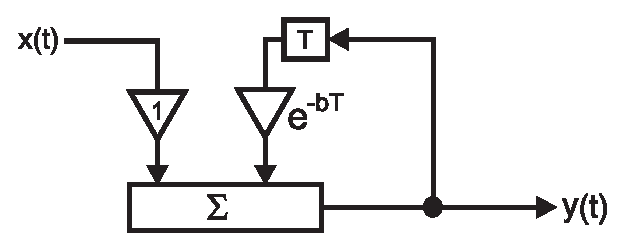
\includegraphics[width=0.75\linewidth]{iir}%
\lthtmlpictureZ
\lthtmlcheckvsize\clearpage}

\stepcounter{subsubsection}
{\newpage\clearpage
\lthtmlinlinemathA{tex2html_wrap_indisplay6607}%
$\displaystyle Y(z)$%
\lthtmlindisplaymathZ
\lthtmlcheckvsize\clearpage}

{\newpage\clearpage
\lthtmlinlinemathA{tex2html_wrap_indisplay6609}%
$\displaystyle X(z)H(z)$%
\lthtmlindisplaymathZ
\lthtmlcheckvsize\clearpage}

{\newpage\clearpage
\lthtmlinlinemathA{tex2html_wrap_indisplay6611}%
$\displaystyle X(z) {1\over 1-e^{-bT} z^{-1}}$%
\lthtmlindisplaymathZ
\lthtmlcheckvsize\clearpage}

{\newpage\clearpage
\lthtmlinlinemathA{tex2html_wrap_indisplay6613}%
$\displaystyle Y(z)z^{-1}e^{-bT}+X(z)$%
\lthtmlindisplaymathZ
\lthtmlcheckvsize\clearpage}

{\newpage\clearpage
\lthtmlinlinemathA{tex2html_wrap_inline2349}%
$z^{-1}$%
\lthtmlindisplaymathZ
\lthtmlcheckvsize\clearpage}

{\newpage\clearpage
\lthtmlinlinemathA{tex2html_wrap_indisplay6617}%
$\displaystyle y(nT)=y([n-1]T) e^{-bT} + x(nT)
$%
\lthtmlindisplaymathZ
\lthtmlcheckvsize\clearpage}

{\newpage\clearpage
\lthtmlinlinemathA{tex2html_wrap_inline2353}%
$y(nT)$%
\lthtmlindisplaymathZ
\lthtmlcheckvsize\clearpage}

{\newpage\clearpage
\lthtmlinlinemathA{tex2html_wrap_inline2355}%
$y([n-1]T)$%
\lthtmlindisplaymathZ
\lthtmlcheckvsize\clearpage}

{\newpage\clearpage
\lthtmlinlinemathA{tex2html_wrap_inline2357}%
$x(nT)$%
\lthtmlindisplaymathZ
\lthtmlcheckvsize\clearpage}

{\newpage\clearpage
\lthtmlinlinemathA{tex2html_wrap_inline2359}%
$e^{-bT}$%
\lthtmlindisplaymathZ
\lthtmlcheckvsize\clearpage}

{\newpage\clearpage
\lthtmlinlinemathA{tex2html_wrap_inline2361}%
$-e^{-bT}$%
\lthtmlindisplaymathZ
\lthtmlcheckvsize\clearpage}

\stepcounter{subsubsection}
{\newpage\clearpage
\lthtmlinlinemathA{tex2html_wrap_indisplay6625}%
$\displaystyle H(z) = \frac{\sum_{k = 0}^{r} B_{k} z^{-k}}{1 + \sum_{l = 1}^{m} A_{i} z^{-l}} $%
\lthtmlindisplaymathZ
\lthtmlcheckvsize\clearpage}

{\newpage\clearpage
\lthtmlinlinemathA{tex2html_wrap_inline2363}%
$B_k$%
\lthtmlindisplaymathZ
\lthtmlcheckvsize\clearpage}

{\newpage\clearpage
\lthtmlinlinemathA{tex2html_wrap_inline2365}%
$A_l$%
\lthtmlindisplaymathZ
\lthtmlcheckvsize\clearpage}

{\newpage\clearpage
\lthtmlpictureA{tex2html_wrap6629}%
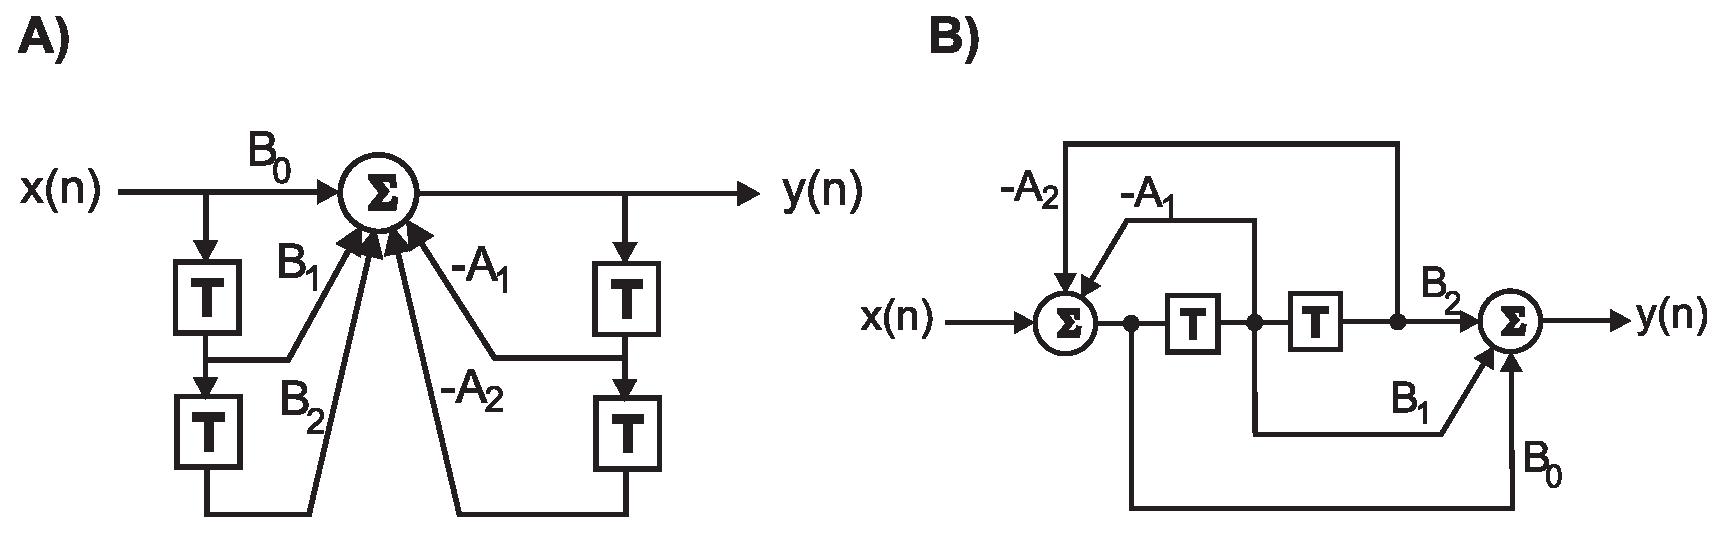
\includegraphics[width=\textwidth]{iir_types}%
\lthtmlpictureZ
\lthtmlcheckvsize\clearpage}

\stepcounter{subsubsection}
{\newpage\clearpage
\lthtmlpictureA{tex2html_wrap6634}%
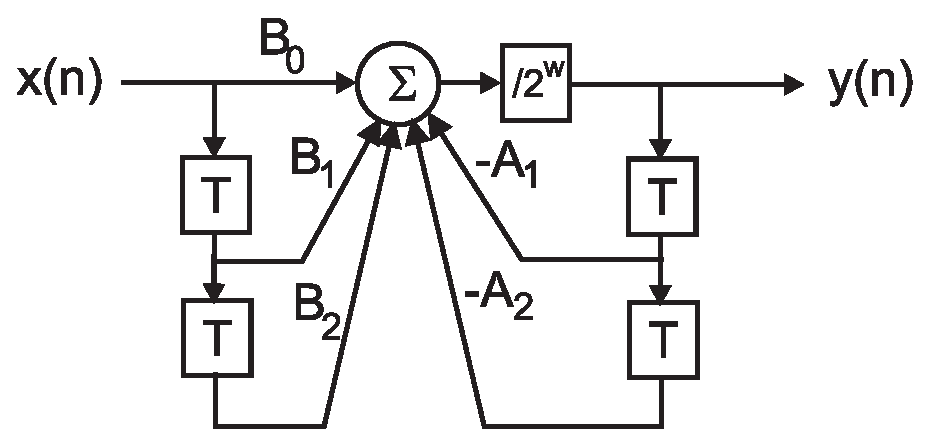
\includegraphics[width=0.5\textwidth]{iir_fixed}%
\lthtmlpictureZ
\lthtmlcheckvsize\clearpage}

\stepcounter{subsubsection}
{\newpage\clearpage
\lthtmlinlinemathA{tex2html_wrap_inline2373}%
$2^{14}$%
\lthtmlindisplaymathZ
\lthtmlcheckvsize\clearpage}

{\newpage\clearpage
\lthtmlinlinemathA{tex2html_wrap_inline2377}%
$14$%
\lthtmlindisplaymathZ
\lthtmlcheckvsize\clearpage}

{\newpage\clearpage
\lthtmlinlinemathA{tex2html_wrap_inline2379}%
$16+14=30$%
\lthtmlindisplaymathZ
\lthtmlcheckvsize\clearpage}

{\newpage\clearpage
\lthtmlpictureA{tex2html_wrap6645}%
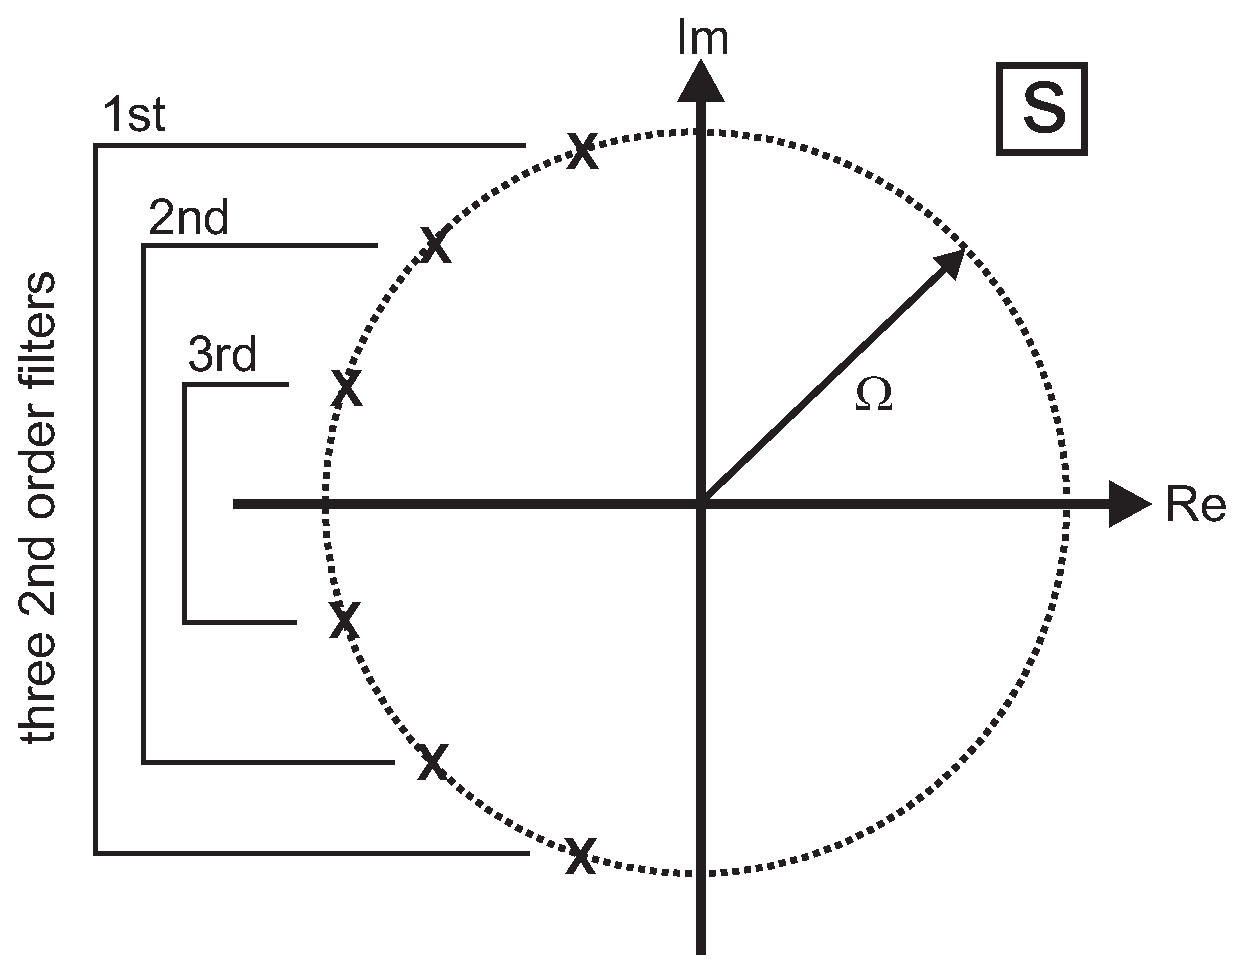
\includegraphics[width=0.5\textwidth]{butterworth_poles}%
\lthtmlpictureZ
\lthtmlcheckvsize\clearpage}

\stepcounter{subsubsection}
{\newpage\clearpage
\lthtmlinlinemathA{tex2html_wrap_inline2385}%
$h(t),H(s)$%
\lthtmlindisplaymathZ
\lthtmlcheckvsize\clearpage}

{\newpage\clearpage
\lthtmlinlinemathA{tex2html_wrap_inline2387}%
$h(n),H(z)$%
\lthtmlindisplaymathZ
\lthtmlcheckvsize\clearpage}

\stepcounter{paragraph}
{\newpage\clearpage
\lthtmlinlinemathA{tex2html_wrap_indisplay6659}%
$\displaystyle |H(\Omega)|^{2} = \frac{1}{1 - \varepsilon^{2} T_{N} (\Omega/\Omega_{p})}
$%
\lthtmlindisplaymathZ
\lthtmlcheckvsize\clearpage}

\stepcounter{paragraph}
\stepcounter{paragraph}
{\newpage\clearpage
\lthtmlinlinemathA{tex2html_wrap_inline2399}%
$0 \ldots \infty$%
\lthtmlindisplaymathZ
\lthtmlcheckvsize\clearpage}

{\newpage\clearpage
\lthtmlinlinemathA{tex2html_wrap_indisplay6669}%
$\displaystyle - \infty < \Omega < \infty \Rightarrow -\pi \leq \omega \leq \pi 
$%
\lthtmlindisplaymathZ
\lthtmlcheckvsize\clearpage}

{\newpage\clearpage
\lthtmlinlinemathA{tex2html_wrap_indisplay6671}%
$\displaystyle s = \frac{2}{T} \quad \frac{z - 1}{z + 1}
$%
\lthtmlindisplaymathZ
\lthtmlcheckvsize\clearpage}

{\newpage\clearpage
\lthtmlinlinemathA{tex2html_wrap_inline2407}%
$\Omega_c$%
\lthtmlindisplaymathZ
\lthtmlcheckvsize\clearpage}

{\newpage\clearpage
\lthtmlinlinemathA{tex2html_wrap_inline2409}%
$s = j\Omega$%
\lthtmlindisplaymathZ
\lthtmlcheckvsize\clearpage}

{\newpage\clearpage
\lthtmlinlinemathA{tex2html_wrap_indisplay6678}%
$\displaystyle j \Omega = \frac{2}{T} \left[\frac{e^{j \omega} - 1}{e^{j \omega} +1}\right] = \frac{2}{T} j \tan \frac{\omega}{2}
$%
\lthtmlindisplaymathZ
\lthtmlcheckvsize\clearpage}

{\newpage\clearpage
\lthtmlinlinemathA{tex2html_wrap_inline2413}%
$j$%
\lthtmlindisplaymathZ
\lthtmlcheckvsize\clearpage}

{\newpage\clearpage
\lthtmlinlinemathA{tex2html_wrap_indisplay6681}%
$\displaystyle \Omega = \frac{2}{T} tan \frac{\omega}{2}
$%
\lthtmlindisplaymathZ
\lthtmlcheckvsize\clearpage}

{\newpage\clearpage
\lthtmlinlinemathA{tex2html_wrap_indisplay6683}%
$\displaystyle \Omega_{c} = \frac{2}{T} tan \frac {\omega_{c}}{2}
$%
\lthtmlindisplaymathZ
\lthtmlcheckvsize\clearpage}

{\newpage\clearpage
\lthtmlinlinemathA{tex2html_wrap_inline2419}%
$\omega_{c} = 2\pi f_{c}$%
\lthtmlindisplaymathZ
\lthtmlcheckvsize\clearpage}

\stepcounter{paragraph}
{\newpage\clearpage
\lthtmlinlinemathA{tex2html_wrap_inline2421}%
$\omega_{c}$%
\lthtmlindisplaymathZ
\lthtmlcheckvsize\clearpage}

{\newpage\clearpage
\lthtmlinlinemathA{tex2html_wrap_inline2423}%
$\omega_{c} \rightarrow
  \Omega_{c}$%
\lthtmlindisplaymathZ
\lthtmlcheckvsize\clearpage}

{\newpage\clearpage
\lthtmlinlinemathA{tex2html_wrap_inline2431}%
$s = \frac{2}{T} \frac{z - 1}{z + 1}$%
\lthtmlindisplaymathZ
\lthtmlcheckvsize\clearpage}

{\newpage\clearpage
\lthtmlinlinemathA{tex2html_wrap_inline2439}%
$z^{-1}, z^{-2}, \ldots$%
\lthtmlindisplaymathZ
\lthtmlcheckvsize\clearpage}

{\newpage\clearpage
\lthtmlinlinemathA{tex2html_wrap_inline2447}%
$H(s) = H_1(s) H_2(s) H_3(s)
\ldots$%
\lthtmlindisplaymathZ
\lthtmlcheckvsize\clearpage}

\stepcounter{paragraph}
\stepcounter{subsection}
{\newpage\clearpage
\lthtmlpictureA{tex2html_wrap6709}%
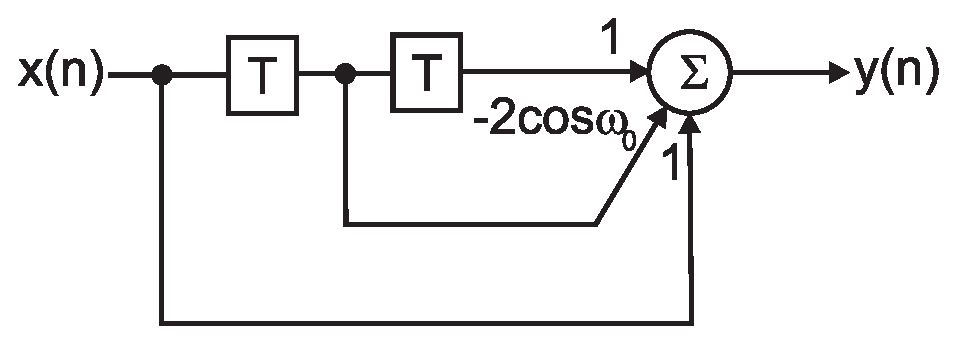
\includegraphics[width=0.75\textwidth]{fir_stop}%
\lthtmlpictureZ
\lthtmlcheckvsize\clearpage}

\stepcounter{subsubsection}
{\newpage\clearpage
\lthtmlinlinemathA{tex2html_wrap_indisplay6719}%
$\displaystyle (1 - e^{j\omega_0} z^{-1})(1 - e^{-j\omega_0} z^{-1})$%
\lthtmlindisplaymathZ
\lthtmlcheckvsize\clearpage}

{\newpage\clearpage
\lthtmlinlinemathA{tex2html_wrap_indisplay6721}%
$\displaystyle 1 - z^{-1} e^{j \omega-{0}} + z^{-2}$%
\lthtmlindisplaymathZ
\lthtmlcheckvsize\clearpage}

{\newpage\clearpage
\lthtmlinlinemathA{tex2html_wrap_indisplay6723}%
$\displaystyle 1 - z^{-1} (e^{j \omega_{0}} + e^{-j \omega_{0}}) + z^{-2}$%
\lthtmlindisplaymathZ
\lthtmlcheckvsize\clearpage}

{\newpage\clearpage
\lthtmlinlinemathA{tex2html_wrap_indisplay6725}%
$\displaystyle 1 - z^{-1} 2 \cos \omega_{0} + z^{-2}$%
\lthtmlindisplaymathZ
\lthtmlcheckvsize\clearpage}

{\newpage\clearpage
\lthtmlinlinemathA{tex2html_wrap_indisplay6727}%
$\displaystyle H(e^{j\omega}) = \underbrace{(1 - e^{j\omega_0}e^{-j\omega})(1 - e^{-j\omega_0} e^{-j\omega})}_{\mbox{2 zeros}}
$%
\lthtmlindisplaymathZ
\lthtmlcheckvsize\clearpage}

{\newpage\clearpage
\lthtmlinlinemathA{tex2html_wrap_inline2453}%
$e^{j \omega_{0}}$%
\lthtmlindisplaymathZ
\lthtmlcheckvsize\clearpage}

{\newpage\clearpage
\lthtmlinlinemathA{tex2html_wrap_inline2455}%
$e^{-j \omega_0}$%
\lthtmlindisplaymathZ
\lthtmlcheckvsize\clearpage}

{\newpage\clearpage
\lthtmlinlinemathA{tex2html_wrap_inline2457}%
$\omega_{0}$%
\lthtmlindisplaymathZ
\lthtmlcheckvsize\clearpage}

{\newpage\clearpage
\lthtmlinlinemathA{tex2html_wrap_inline2459}%
$-\omega_{0}$%
\lthtmlindisplaymathZ
\lthtmlcheckvsize\clearpage}

{\newpage\clearpage
\lthtmlinlinemathA{tex2html_wrap_inline2461}%
$\omega_{0} = 0$%
\lthtmlindisplaymathZ
\lthtmlcheckvsize\clearpage}

{\newpage\clearpage
\lthtmlinlinemathA{tex2html_wrap_indisplay6736}%
$\displaystyle (1 - e^{0} z^{-1})(1 - e^{0} z^{-1})$%
\lthtmlindisplaymathZ
\lthtmlcheckvsize\clearpage}

{\newpage\clearpage
\lthtmlinlinemathA{tex2html_wrap_indisplay6738}%
$\displaystyle 1 - 2 z^{-1} + z^{-2}$%
\lthtmlindisplaymathZ
\lthtmlcheckvsize\clearpage}

{\newpage\clearpage
\lthtmlpictureA{tex2html_wrap6739}%
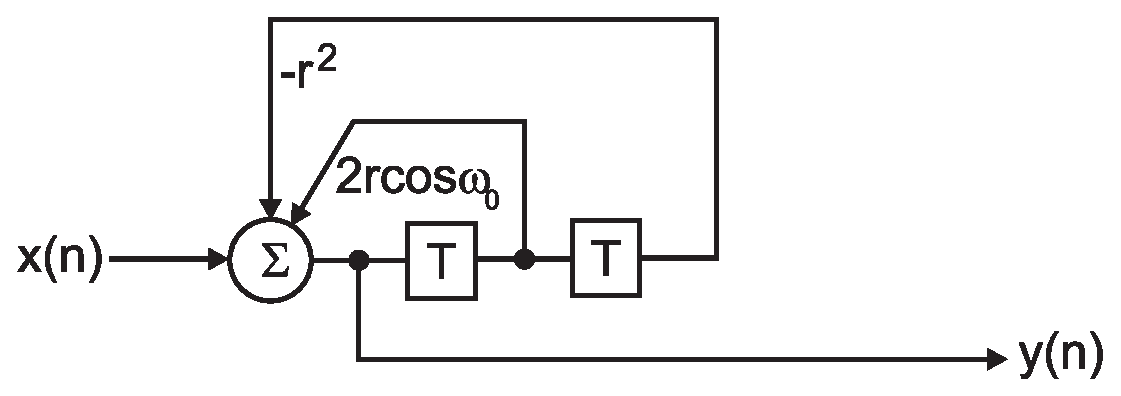
\includegraphics[width=0.75\textwidth]{iir_stop}%
\lthtmlpictureZ
\lthtmlcheckvsize\clearpage}

\stepcounter{subsubsection}
{\newpage\clearpage
\lthtmlinlinemathA{tex2html_wrap_indisplay6749}%
$\displaystyle H(z) = \frac{1}{\underbrace{(1 - r e^{j \omega_{0}} z^{-1})(1 - r e^{-j \omega_{0}} z^{-1})}_{2 poles!}}
$%
\lthtmlindisplaymathZ
\lthtmlcheckvsize\clearpage}

{\newpage\clearpage
\lthtmlinlinemathA{tex2html_wrap_inline2469}%
$0<r<1$%
\lthtmlindisplaymathZ
\lthtmlcheckvsize\clearpage}

{\newpage\clearpage
\lthtmlinlinemathA{tex2html_wrap_indisplay6754}%
$\displaystyle H(z) = \frac{1}{1 - 2 r \cos(\omega_{0}) z^{-1} + r^{2} z^{-2}} 
$%
\lthtmlindisplaymathZ
\lthtmlcheckvsize\clearpage}

{\newpage\clearpage
\lthtmlinlinemathA{tex2html_wrap_inline2473}%
$Y(z)$%
\lthtmlindisplaymathZ
\lthtmlcheckvsize\clearpage}

{\newpage\clearpage
\lthtmlinlinemathA{tex2html_wrap_indisplay6759}%
$\displaystyle X(z) \frac{1}{1 - 2 r \cos (\omega) z^{-1} + r^{2} z^{-2}}$%
\lthtmlindisplaymathZ
\lthtmlcheckvsize\clearpage}

{\newpage\clearpage
\lthtmlinlinemathA{tex2html_wrap_indisplay6760}%
$\displaystyle X(z)$%
\lthtmlindisplaymathZ
\lthtmlcheckvsize\clearpage}

{\newpage\clearpage
\lthtmlinlinemathA{tex2html_wrap_indisplay6762}%
$\displaystyle Y(z) - Y(z) 2r \cos (\omega_{0}) z^{-1} + Y(z) r^{2} z^{-2}$%
\lthtmlindisplaymathZ
\lthtmlcheckvsize\clearpage}

{\newpage\clearpage
\lthtmlinlinemathA{tex2html_wrap_indisplay6765}%
$\displaystyle X(z) + z^{-1} Y(z) 2r \cos (\omega_{0}) - z^{-2} Y(z) r^{2}$%
\lthtmlindisplaymathZ
\lthtmlcheckvsize\clearpage}

{\newpage\clearpage
\lthtmlinlinemathA{tex2html_wrap_inline2475}%
$\pm\omega_0$%
\lthtmlindisplaymathZ
\lthtmlcheckvsize\clearpage}

\stepcounter{subsubsection}
{\newpage\clearpage
\lthtmlinlinemathA{tex2html_wrap_inline2485}%
$r>1$%
\lthtmlindisplaymathZ
\lthtmlcheckvsize\clearpage}

{\newpage\clearpage
\lthtmlinlinemathA{tex2html_wrap_inline2487}%
$-1
\ldots +1$%
\lthtmlindisplaymathZ
\lthtmlcheckvsize\clearpage}

\stepcounter{subsubsection}
{\newpage\clearpage
\lthtmlinlinemathA{tex2html_wrap_indisplay6783}%
$\displaystyle H(z) = \frac {1 - 2 \cos (\omega_{0}) z^{-1} + z^{-2}}{1 - 2r \cos (\omega_{0}) z^{-1} + r^{2} z^{-2}} 
$%
\lthtmlindisplaymathZ
\lthtmlcheckvsize\clearpage}

{\newpage\clearpage
\lthtmlinlinemathA{tex2html_wrap_inline2493}%
$r<1$%
\lthtmlindisplaymathZ
\lthtmlcheckvsize\clearpage}

\stepcounter{subsubsection}
\stepcounter{section}
{\newpage\clearpage
\lthtmlinlinemathA{tex2html_wrap_indisplay6795}%
$\displaystyle H(z) = \frac{b}{1 - a z^{-1}}
$%
\lthtmlindisplaymathZ
\lthtmlcheckvsize\clearpage}

{\newpage\clearpage
\lthtmlinlinemathA{tex2html_wrap_inline2509}%
$a$%
\lthtmlindisplaymathZ
\lthtmlcheckvsize\clearpage}

{\newpage\clearpage
\lthtmlinlinemathA{tex2html_wrap_indisplay6798}%
$\displaystyle |H(e^{j \omega}) | = |\frac{b}{1 - a e^{-j \omega}}| 
$%
\lthtmlindisplaymathZ
\lthtmlcheckvsize\clearpage}

{\newpage\clearpage
\lthtmlinlinemathA{tex2html_wrap_indisplay6800}%
$\displaystyle \underbrace{y(n)}_{\mbox {\footnotesize actual estimate}} = a(n) \underbrace{y(n - 1)}_{\mbox{\footnotesize previous estimate}} + b(n)\underbrace{x(n)}_{\mbox{\footnotesize current data sample}} 
$%
\lthtmlindisplaymathZ
\lthtmlcheckvsize\clearpage}

{\newpage\clearpage
\lthtmlinlinemathA{tex2html_wrap_indisplay6803}%
$\displaystyle p(n) = E[ \left( y (k) - y_{real} (k)\right)^{2}] 
$%
\lthtmlindisplaymathZ
\lthtmlcheckvsize\clearpage}

{\newpage\clearpage
\lthtmlinlinemathA{tex2html_wrap_inline2513}%
$p$%
\lthtmlindisplaymathZ
\lthtmlcheckvsize\clearpage}


\end{document}
